%%%%%%%%%%%%%%%%%%%%%%%%%%%%% Thesis.tex %%%%%%%%%%%%%%%%%%%%%%%%%%%%%%%
%                                                                      %
%  ---------- Master of Science Dissertation template ----------       %
%                                                                      %
%  Template for the Master Thesis according to the regulations         %
%  published by the Academic Board (Direcção Académica) at IST.        %
%                                                                      %
%  For up-to-date guide, please refer to the official website          %
%  http://academica.tecnico.ulisboa.pt/alunos/dissertacao-de-mestrado/ %
%                                                                      %
%       Andre C. Marta                                                 %
%       Area Cientifica de Mecanica Aplicada e Aeroespacial            %
%       Departamento de Engenharia Mecanica                            %
%       Instituto Superior Tecnico                                     %
%       Av. Rovisco Pais                                               %
%       1049-001 Lisboa                                                %
%       Portugal                                                       %
%       Tel: +351 21 841 9469                                          %
%                        3469 (extension)                              %
%       Email: andre.marta@tecnico.ulisboa.pt                          %
%                                                                      %
%  Created:       Jan 20, 2011                                         %
%  Last Modified: Feb 19, 2018                                         %
%                                                                      %
%%%%%%%%%%%%%%%%%%%%%%%%%%%%%%%%%%%%%%%%%%%%%%%%%%%%%%%%%%%%%%%%%%%%%%%%
%  Revision history                                                    %
%  v1 - 2011/01/24 - original template                                 %
%  v2 - 2012/10/30 - new IST image and glossary support                %
%  v3 - 2013/12/10 - update according to 2012/13 official guide        %
%  v4 - 2014/02/28 - new default for bibliography style                %
%  v5 - 2014/05/07 - update according to 2013/14 official guide        %
%  v6 - 2015/07/02 - cover page format fixed,                          %
%                    contents page numbering fixed,                    %
%                    better language support,                          %
%                    enhanced examples of tables,                      %
%                    new option for appendix page numbering format,    %
%                    custom bibliography style                         %
%  v7 - 2018/02/19 - multiple citations compressed                     %
%%%%%%%%%%%%%%%%%%%%%%%%%%%%%%%%%%%%%%%%%%%%%%%%%%%%%%%%%%%%%%%%%%%%%%%%
%                                                                      %
% To generate the PDF file, type "make" at the terminal prompt.        %
%                                                                      %
% The IST template LaTeX package was created by the author             %
% and it can be downloaded from:                                       %
% https://fenix.ist.utl.pt/homepage/ist31052/                          %
%                                                                      %
% The external packages can be downloaded from                         %
% the Comprehensive TeX Archive Network at http://www.ctan.org/        %
%                                                                      %
% List of LaTex symbols:                                               %
% http://www.ctan.org/tex-archive/info/symbols/comprehensive/          %
%                                                                      %
% Help with LaTex can be found at                                      %
% http://www.giss.nasa.gov/tools/latex/ltx-2.html                      %
% http://en.wikibooks.org/wiki/LaTeX                                   %
%%%%%%%%%%%%%%%%%%%%%%%%%%%%%%%%%%%%%%%%%%%%%%%%%%%%%%%%%%%%%%%%%%%%%%%%

%%%%%%%%%%%%%%%%%%%%%%%%%%%%%%%%%%%%%%%%%%%%%%%%%%%%%%%%%%%%%%%%%%%%%%%%
%     Preamble                                                         %
%%%%%%%%%%%%%%%%%%%%%%%%%%%%%%%%%%%%%%%%%%%%%%%%%%%%%%%%%%%%%%%%%%%%%%%%

% ----------------------------------------------------------------------
%  Set the document class
% ----------------------------------------------------------------------
\documentclass[10pt,a4paper,twoside]{report}

% ----------------------------------------------------------------------
% Define external packages, language, margins, fonts and new commands
% ----------------------------------------------------------------------
%%%%%%%%%%%%%%%%%%%%%%%%%%%%%%%%%%%%%%%%%%%%%%%%%%%%%%%%%%%%%%%%%%%%%%%%
%                                                                      %
%     File: Thesis_Preamble.tex                                        %
%     Tex Master: Thesis.tex                                           %
%                                                                      %
%     Author: Gonçalo Santos                                           %
%     Last modified : 20 Oct 2018                                      %
%                                                                      %
%%%%%%%%%%%%%%%%%%%%%%%%%%%%%%%%%%%%%%%%%%%%%%%%%%%%%%%%%%%%%%%%%%%%%%%%

% ----------------------------------------------------------------------
% Define document language.
% ----------------------------------------------------------------------

% 'inputenc' package
%
% Accept different input encodings.
% http://www.ctan.org/tex-archive/macros/latex/base/
%
% > allows typing non-english text in LaTeX sources.
%
% ******************************* SELECT *******************************
%\usepackage[latin1]{inputenc} % <<<<< Windows
\usepackage[utf8]{inputenc}   % <<<<< Linux
% ******************************* SELECT *******************************


% 'babel' package
%
% Multilingual support for Plain TeX or LaTeX.
% http://www.ctan.org/tex-archive/macros/latex/required/babel/
%
% > sets the variable names according to the language selected
%
% ******************************* SELECT *******************************
%\usepackage[portuguese]{babel} % <<<<< Portuguese
\usepackage[english]{babel} % <<<<< English
% ******************************* SELECT *******************************


% List of LaTeX variable names: \abstractname, \appendixname, \bibname,
%   \chaptername, \contentsname, \listfigurename, \listtablename, ...
% http://www.tex.ac.uk/cgi-bin/texfaq2html?label=fixnam
%
% Changing the words babel uses (uncomment and redefine as necessary...)
%
\newcommand{\acknowledgments}{@undefined} % new LaTeX variable name
%
% > English
%
\addto\captionsenglish{\renewcommand{\acknowledgments}{Acknowledgments}}
%\addto\captionsenglish{\renewcommand{\listtablename}{List of Tables}}
%\addto\captionsenglish{\renewcommand{\listfigurename}{List of Figures}}
%\addto\captionsenglish{\renewcommand{\nomname}{Nomenclature}}
%\addto\captionsenglish{\renewcommand{\appendixname}{Appendix}}
%\addto\captionsenglish{\renewcommand{\bibname}{References}} % Bibliography

% > Portuguese
%
\addto\captionsportuguese{\renewcommand{\acknowledgments}{Agradecimentos}}
%\addto\captionsportuguese{\renewcommand{\listtablename}{Lista de Figuras}}
%\addto\captionsportuguese{\renewcommand{\listfigurename}{Lista de Tabelas}}
\addto\captionsportuguese{\renewcommand{\nomname}{Lista de S\'{i}mbolos}} % Nomenclatura
%\addto\captionsportuguese{\renewcommand{\appendixname}{Anexo}} % Apendice
%\addto\captionsportuguese{\renewcommand{\bibname}{Refer\^{e}ncias}} % Bibliografia


% ----------------------------------------------------------------------
% Define default and cover page fonts.
% ----------------------------------------------------------------------

% Use Arial font as default
%
\renewcommand{\rmdefault}{phv}
\renewcommand{\sfdefault}{phv}

% Define cover page fonts
%
%         encoding     family       series      shape
%  \usefont{T1}     {phv}=helvetica  {b}=bold    {n}=normal
%                   {ptm}=times      {m}=normal  {sl}=slanted
%                                                {it}=italic
% see more examples at
% http://julien.coron.free.fr/languages/latex/fonts/
%
\def\FontLn{% 16 pt normal
  \usefont{T1}{phv}{m}{n}\fontsize{16pt}{16pt}\selectfont}
\def\FontLb{% 16 pt bold
  \usefont{T1}{phv}{b}{n}\fontsize{16pt}{16pt}\selectfont}
\def\FontMn{% 14 pt normal
  \usefont{T1}{phv}{m}{n}\fontsize{14pt}{14pt}\selectfont}
\def\FontMb{% 14 pt bold
  \usefont{T1}{phv}{b}{n}\fontsize{14pt}{14pt}\selectfont}
\def\FontSn{% 12 pt normal
  \usefont{T1}{phv}{m}{n}\fontsize{12pt}{12pt}\selectfont}


% ----------------------------------------------------------------------
% Define page margins and line spacing.
% ----------------------------------------------------------------------

% 'geometry' package
%
% Flexible and complete interface to document dimensions.
% http://www.ctan.org/tex-archive/macros/latex/contrib/geometry/
%
% > set the page margins (2.5cm minimum in every side, as per IST rules)
%
\usepackage{geometry}	
\geometry{verbose,tmargin=2.5cm,bmargin=2.5cm,lmargin=2.5cm,rmargin=2.5cm}

% 'setspace' package
%
% Set space between lines.
% http://www.ctan.org/tex-archive/macros/latex/contrib/setspace/
%
% > allow setting line spacing (line spacing of 1.5, as per IST rules)
%
\usepackage{setspace}
\renewcommand{\baselinestretch}{1.5}


% ----------------------------------------------------------------------
% Include external packages.
% Note that not all of these packages may be available on all system
% installations. If necessary, include the .sty files locally in
% the <jobname>.tex file directory.
% ----------------------------------------------------------------------

% 'graphicx' package
%
% Enhanced support for graphics.
% http://www.ctan.org/tex-archive/macros/latex/required/graphics/
%
% > extends arguments of the \includegraphics command
%
\usepackage{graphicx}


% 'color' package
%
% Colour control for LaTeX documents.
% http://www.ctan.org/tex-archive/macros/latex/required/graphics/
%
% > defines color macros: \color{<color name>}
%
%\usepackage{color}


% 'amsmath' package
%
% Mathematical enhancements for LaTeX.
% http://www.ctan.org/tex-archive/macros/latex/required/amslatex/
%
% > American Mathematical Society plain Tex macros
%
\usepackage{amsmath}  % AMS mathematical facilities for LaTeX.
\usepackage{amsthm}   % Typesetting theorems (AMS style).
\usepackage{amsfonts} %


% 'wrapfig' package
%
% Produces figures which text can flow around.
% http://www.ctan.org/tex-archive/macros/latex/contrib/wrapfig/
%
% > wrap figures/tables in text (i.e., Di Vinci style)
%
% \usepackage{wrapfig}


% 'subfigure' package
%
% Deprecated: Figures divided into subfigures.
% http://www.ctan.org/tex-archive/obsolete/macros/latex/contrib/subfigure/
%
% > subcaptions for subfigures
%
\usepackage{subfigure}


% 'subfigmat' package
%
% Automates layout when using the subfigure package.
% http://www.ctan.org/tex-archive/macros/latex/contrib/subfigmat/
%
% > matrices of similar subfigures
%
\usepackage{subfigmat}


% 'url' package
%
% Verbatim with URL-sensitive line breaks.
% http://www.ctan.org/tex-archive/macros/latex/contrib/url/
%
% > URLs in BibTex
%
% \usepackage{url}


% 'varioref' package
%
% Intelligent page references.
% http://www.ctan.org/tex-archive/macros/latex/required/tools/
%
% > smart page, figure, table and equation referencing
%
%\usepackage{varioref}


% 'dcolumn' package
%
% Align on the decimal point of numbers in tabular columns.
% http://www.ctan.org/tex-archive/macros/latex/required/tools/
%
% > decimal-aligned tabular math columns
%
\usepackage{dcolumn}
\newcolumntype{d}{D{.}{.}{-1}} % column aligned by the point separator '.'
\newcolumntype{e}{D{E}{E}{-1}} % column aligned by the exponent 'E'


% '' package
%
% Reimplementation of and extensions to LaTeX verbatim.
% http://www.ctan.org/tex-archive/macros/latex/required/tools/
%
% > provides the verbatim environment (\begin{verbatim},\end{verbatim})
%   and a comment environment (\begin{comment},  \end{comment})
%
% \usepackage{verbatim}


% 'moreverb' package
%
% Extended verbatim.
% http://www.ctan.org/tex-archive/macros/latex/contrib/moreverb/
%
% > supports tab expansion and line numbering
%
% \usepackage{moreverb}



% 'nomencl' package
%
% Produce lists of symbols as in nomenclature.
% http://www.ctan.org/tex-archive/macros/latex/contrib/nomencl/
%
% The nomencl package makes use of the MakeIndex program
% in order to produce the nomenclature list.
%
% Nomenclature
% 1: On running the file through LATEX, the command \makenomenclature
%    in the preamble instructs it to create/open the nomenclature file
%    <jobname>.nlo corresponding to the LATEX file <jobname>.tex and
%    writes the information from the \nomenclature commands to this file.
% 2: The next step is to invoke MakeIndex in order to produce the
%    <jobname>.nls file. This can be achieved by making use of the
%    command: makeindex <jobname>.nlo -s nomencl.ist -o <jobname>.nls
% 3: The last step is to invoke LATEX on the <jobname>.tex file once
%    more. There, the \printnomenclature in the document will input the
%    <jobname>.nls file and process it according to the given options.
%
% http://www-h.eng.cam.ac.uk/help/tpl/textprocessing/nomencl.pdf
%
% Nomenclature (produces *.nlo *.nls files)
\usepackage{nomencl}
\makenomenclature
%
% Group variables according to their symbol type
%
\RequirePackage{ifthen}
\ifthenelse{\equal{\languagename}{english}}%
    { % English
    \renewcommand{\nomgroup}[1]{%
      \ifthenelse{\equal{#1}{R}}{%
        \item[\textbf{Roman symbols}]}{%
        \ifthenelse{\equal{#1}{G}}{%
          \item[\textbf{Greek symbols}]}{%
          \ifthenelse{\equal{#1}{S}}{%
            \item[\textbf{Subscripts}]}{%
            \ifthenelse{\equal{#1}{T}}{%
              \item[\textbf{Superscripts}]}{}}}}}%
    }{% Portuguese
    \renewcommand{\nomgroup}[1]{%
      \ifthenelse{\equal{#1}{R}}{%
        \item[\textbf{Simbolos romanos}]}{%
        \ifthenelse{\equal{#1}{G}}{%
          \item[\textbf{Simbolos gregos}]}{%
          \ifthenelse{\equal{#1}{S}}{%
            \item[\textbf{Subscritos}]}{%
            \ifthenelse{\equal{#1}{T}}{%
              \item[\textbf{Sobrescritos}]}{}}}}}%
    }%


% 'glossary' package
%
% Create a glossary.
% http://www.ctan.org/tex-archive/macros/latex/contrib/glossary/
%
% Glossary (produces *.glo *.ist files)
\usepackage[number=none]{glossary}
% (remove blank line between groups)
\setglossary{gloskip={}}
% (redefine glossary style file)
%\renewcommand{\istfilename}{myGlossaryStyle.ist}
\makeglossary


% 'rotating' package
%
% Rotation tools, including rotated full-page floats.
% http://www.ctan.org/tex-archive/macros/latex/contrib/rotating/
%
% > show wide figures and tables in landscape format:
%   use \begin{sidewaystable} and \begin{sidewaysfigure}
%   instead of 'table' and 'figure', respectively.
%
\usepackage{rotating}


% 'hyperref' package
%
% Extensive support for hypertext in LaTeX.
% http://www.ctan.org/tex-archive/macros/latex/contrib/hyperref/
%
% > Extends the functionality of all the LATEX cross-referencing
%   commands (including the table of contents, bibliographies etc) to
%   produce \special commands which a driver can turn into hypertext
%   links; Also provides new commands to allow the user to write adhoc
%   hypertext links, including those to external documents and URLs.
%
\usepackage[pdftex]{hyperref} % enhance documents that are to be
                              % output as HTML and PDF
\hypersetup{colorlinks,       % color text of links and anchors,
                              % eliminates borders around links
%            linkcolor=red,    % color for normal internal links
            linkcolor=black,  % color for normal internal links
            anchorcolor=black,% color for anchor text
%            citecolor=green,  % color for bibliographical citations
            citecolor=black,  % color for bibliographical citations
%            filecolor=magenta,% color for URLs which open local files
            filecolor=black,  % color for URLs which open local files
%            menucolor=red,    % color for Acrobat menu items
            menucolor=black,  % color for Acrobat menu items
%            pagecolor=red,    % color for links to other pages
            pagecolor=black,  % color for links to other pages
%            urlcolor=cyan,    % color for linked URLs
            urlcolor=black,   % color for linked URLs
	          bookmarks=true,         % create PDF bookmarks
	          bookmarksopen=false,    % don't expand bookmarks
	          bookmarksnumbered=true, % number bookmarks
	          pdftitle={Thesis},
            pdfauthor={Andre C. Marta},
            pdfsubject={Thesis Title},
            pdfkeywords={Thesis Keywords},
            pdfstartview=FitV,
            pdfdisplaydoctitle=true}


% 'hypcap' package
%
% Adjusting the anchors of captions.
% http://www.ctan.org/tex-archive/macros/latex/contrib/oberdiek/
%
% > fixes the problem with hyperref, that links to floats points
%   below the caption and not at the beginning of the float.
%
\usepackage[figure,table]{hypcap}


% 'natbib' package
%
% Flexible bibliography support.
% http://www.ctan.org/tex-archive/macros/latex/contrib/natbib/
%
% > produce author-year style citations
%
% \citet  and \citep  for textual and parenthetical citations, respectively
% \citet* and \citep* that print the full author list, and not just the abbreviated one
% \citealt is the same as \citet but without parentheses. Similarly, \citealp is \citep without parentheses
% \citeauthor
% \citeyear
% \citeyearpar
%
\usepackage{natbib}


% ----------------------------------------------------------------------
% Define new commands to assure consistent treatment throughout document
% ----------------------------------------------------------------------

\newcommand{\ud}{\mathrm{d}}                % total derivative
\newcommand{\degree}{\ensuremath{^\circ\,}} % degrees

% Abbreviations

\newcommand{\mcol}{\multicolumn}            % table format

\newcommand{\eqnref}[1]{(\ref{#1})}
\newcommand{\class}[1]{\texttt{#1}}
\newcommand{\package}[1]{\texttt{#1}}
\newcommand{\file}[1]{\texttt{#1}}
\newcommand{\BibTeX}{\textsc{Bib}\TeX}

% Typefaces ( example: {\bf Bold text here} )
%
% > pre-defined
%   \bf % bold face
%   \it % italic
%   \tt % typewriter
%
% > newly defined
\newcommand{\tr}[1]{{\ensuremath{\textrm{#1}}}}   % text roman
\newcommand{\tb}[1]{{\ensuremath{\textbf{#1}}}}   % text bold face
\newcommand{\ti}[1]{{\ensuremath{\textit{#1}}}}   % text italic
\newcommand{\mc}[1]{{\ensuremath{\mathcal{#1}}}}  % math calygraphy
\newcommand{\mco}[1]{{\ensuremath{\mathcalold{#1}}}}% math old calygraphy
\newcommand{\mr}[1]{{\ensuremath{\mathrm{#1}}}}   % math roman
\newcommand{\mb}[1]{{\ensuremath{\mathbf{#1}}}}   % math bold face
\newcommand{\bs}[1]{\ensuremath{\boldsymbol{#1}}} % math symbol
\def\bm#1{\mathchoice                             % math bold
  {\mbox{\boldmath$\displaystyle#1$}}%
  {\mbox{\boldmath$#1$}}%
  {\mbox{\boldmath$\scriptstyle#1$}}%
  {\mbox{\boldmath$\scriptscriptstyle#1$}}}
\newcommand{\boldcal}[1]{{\ensuremath{\boldsymbol{\mathcal{#1}}}}}% math bold calygraphy

\usepackage{fancyvrb}
 % file "Thesis_Preamble.tex"

%%%%%%%%%%%%%%%%%%%%%%%%%%%%%%%%%%%%%%%%%%%%%%%%%%%%%%%%%%%%%%%%%%%%%%%%
%     Begin Document                                                   %
%%%%%%%%%%%%%%%%%%%%%%%%%%%%%%%%%%%%%%%%%%%%%%%%%%%%%%%%%%%%%%%%%%%%%%%%
\begin{document}

% Set plain page style (no headers, footer with centered page number)
\pagestyle{plain}

% Set roman numbering (i,ii,...) before the start of chapters
\pagenumbering{roman}

% ----------------------------------------------------------------------
%  Cover page
% ----------------------------------------------------------------------
%%%%%%%%%%%%%%%%%%%%%%%%%%%%%%%%%%%%%%%%%%%%%%%%%%%%%%%%%%%%%%%%%%%%%%%%
%                                                                      %
%     File: Thesis_FrontCover.tex                                      %
%     Tex Master: Thesis.tex                                           %
%                                                                      %
%     Author: Gonçalo Santos                                           %
%     Last modified : 20 Oct 2018                                      %
%                                                                      %
%%%%%%%%%%%%%%%%%%%%%%%%%%%%%%%%%%%%%%%%%%%%%%%%%%%%%%%%%%%%%%%%%%%%%%%%

\thispagestyle {empty}

% IST Logo
% parameters: bb=llx lly urx ury (bounding box), width=h_length, height=v_length, angle=angle, scale=factor, clip=true/false, draft=true/false.
\vspace*{-12mm}
\hspace*{-12mm}

\includegraphics[height=20mm]{IST_A_CMYK_POS-crop.pdf}

\begin{center}
%
% Figure (Image or plot)
\vspace{0.5cm}
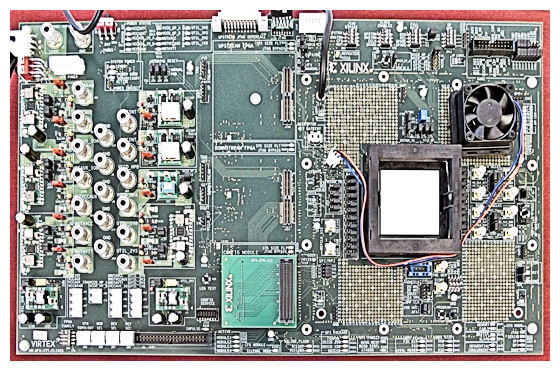
\includegraphics[height=60mm]{Figures/fpga.jpg}

% Title, author and degree
\vspace{0.8cm}
{\FontLb C Compiler for the VERSAT Reconfigurable Processor} \\
\vspace{3.6cm}
{\FontMb Gonçalo da Conceição Reis dos Santos} \\
\vspace{1.9cm}
{\FontLn Thesis to obtain the Master of Science Degree in} \\
\vspace{0.3cm}
{\FontLb Electrical and Computer Engineering} \\
%\vspace{1.9cm}
\vspace{1.0cm}
{\FontSn %
\begin{tabular}{ll}
Supervisor: & Prof. José João Henriques Teixeira de Sousa
\end{tabular} } \\
\vspace{1.0cm}
{\FontMb Examination Committee} \\
\vspace{0.3cm}
{\FontSn %
\begin{tabular}{ll}
Chairperson: & Prof. Francisco André Corrêa Alegria\\
Supervisor: & Prof. José João Henriques Teixeira de Sousa \\
Member of the Committee: & Prof. Paulo Ferreira Godinho Flores \\
\end{tabular} } \\
\vspace{1.5cm}
{\FontMb November 2019} \\
%
\end{center}

\cleardoublepage
 % file "Thesis_FrontCover.tex"
\cleardoublepage

% ----------------------------------------------------------------------
% Dedication page (optional)
% ----------------------------------------------------------------------
%%%%%%%%%%%%%%%%%%%%%%%%%%%%%%%%%%%%%%%%%%%%%%%%%%%%%%%%%%%%%%%%%%%%%%%%%
%                                                                      %
%     File: Thesis_Dedication.tex                                      %
%     Tex Master: Thesis.tex                                           %
%                                                                      %
%     Author: Andre C. Marta                                           %
%     Last modified :  2 Jul 2015                                      %
%                                                                      %
%%%%%%%%%%%%%%%%%%%%%%%%%%%%%%%%%%%%%%%%%%%%%%%%%%%%%%%%%%%%%%%%%%%%%%%%

\null\vskip5cm%
\begin{flushright}
     Dedicated to someone special...
\end{flushright}
\vfill\newpage

 % file "Thesis_Dedication.tex"
%\cleardoublepage

% ----------------------------------------------------------------------
%  Acknowledgments (optional)
% ----------------------------------------------------------------------
%%%%%%%%%%%%%%%%%%%%%%%%%%%%%%%%%%%%%%%%%%%%%%%%%%%%%%%%%%%%%%%%%%%%%%%%%
%                                                                      %
%     File: Thesis_Acknowledgments.tex                                 %
%     Tex Master: Thesis.tex                                           %
%                                                                      %
%     Author: Andre C. Marta                                           %
%     Last modified :  2 Jul 2015                                      %
%                                                                      %
%%%%%%%%%%%%%%%%%%%%%%%%%%%%%%%%%%%%%%%%%%%%%%%%%%%%%%%%%%%%%%%%%%%%%%%%

\section*{\acknowledgments}

% Add entry in the table of contents as section
\addcontentsline{toc}{section}{\acknowledgments}

I want to thank my supervisor, Professor José Teixeira de Sousa, for the 
opportunity to develop this work and for his guidance and support during that process. 
His help was fundamental to overcome the multiple obstacles that I faced during this work.

I also want to acknowledge Professor Horácio Neto for providing a simple Convolutional 
Neural Network application, used as a basis for the application developed for the 
RV32-Versat architecture.

A special acknowledgement goes to my friends, for their continuous support, and Válter,  
that is developing a multi-layer architecture for RV32-Versat. When everything seemed to 
be doomed he always had a miraculous solution.

Finally, I want to express my sincere gratitude to my family for giving me all the 
support and encouragement that I needed throughout my years of study and through the 
process of researching and writing this thesis. They are also part of this work.\\

\textbf{Thank you.}

 % file "Thesis_Acknowledgements.tex"
%\cleardoublepage

% ----------------------------------------------------------------------
%  Abstract (both in English and Portuguese)
% ----------------------------------------------------------------------
%%%%%%%%%%%%%%%%%%%%%%%%%%%%%%%%%%%%%%%%%%%%%%%%%%%%%%%%%%%%%%%%%%%%%%%%%
%                                                                      %
%     File: Thesis_Resumo.tex                                          %
%     Tex Master: Thesis.tex                                           %
%                                                                      %
%     Author: Carlos A. Rodrigues                                           %
%     Last modified : 21 Jan 2011                                      %
%                                                                      %
%%%%%%%%%%%%%%%%%%%%%%%%%%%%%%%%%%%%%%%%%%%%%%%%%%%%%%%%%%%%%%%%%%%%%%%%

\section*{Resumo}

% Add entry in the table of contents as section
\addcontentsline{toc}{section}{Resumo}

Inserir o resumo em Portugu\^{e}s aqui com o máximo de 250 palavras e acompanhado de 4 a 6 palavras-chave...

\vfill

\textbf{\Large Palavras-chave:} OpenRISC, Sistema em um chip,...

\cleardoublepage

   % file "Thesis_Resumo.tex"
%\cleardoublepage

%%%%%%%%%%%%%%%%%%%%%%%%%%%%%%%%%%%%%%%%%%%%%%%%%%%%%%%%%%%%%%%%%%%%%%%%
%                                                                      %
%     File: Thesis_Abstract.tex                                        %
%     Tex Master: Thesis.tex                                           %
%                                                                      %
%     Author: Andre C. Marta                                           %
%     Last modified :  2 Jul 2015                                      %
%                                                                      %
%%%%%%%%%%%%%%%%%%%%%%%%%%%%%%%%%%%%%%%%%%%%%%%%%%%%%%%%%%%%%%%%%%%%%%%%

\section*{Abstract}

% Add entry in the table of contents as section
\addcontentsline{toc}{section}{Abstract}

Versat is a Coarse-Grain Reconfigurable Array architecture (CGRA), which
implements self and partial reconfiguration by using a simple controller
unit. This report studies the current state of the art in HDL and CGRA
simulation, providing a basis to the development of a simulation environment for
Versat. The main objective of this environment is to provide a faster way to
develop and debug software without the use of prototyping hardware. Therefore,
the two types of HDL simulators, event-driven and cycle-accurate, their
advantages and disadvantages are studied, along with a performance comparison
between them. A study of high-level implementations for CGRA simulation is
also presented.

\vfill

\textbf{\Large Keywords:} Versat, coarse-grain reconfigurable arrays, HDL
simulation, CGRA simulation, high-level simulation

 % file "Thesis_Abstract.tex"
\cleardoublepage

% ----------------------------------------------------------------------
%  Table of contents, list of tables, list of figures and nomenclature
% ----------------------------------------------------------------------

% Table of contents
%
\tableofcontents
\cleardoublepage 

% List of tables
%
% Add entry in the table of contents as section
\phantomsection
\addcontentsline{toc}{section}{\listtablename}
% Generate list
\listoftables
\cleardoublepage 

% List of figures
%
% Add entry in the table of contents as section
\phantomsection
\addcontentsline{toc}{section}{\listfigurename}
% Generate list
\listoffigures
\cleardoublepage 

% Nomenclature
%
% entries of nomenclature list
%%%%%%%%%%%%%%%%%%%%%%%%%%%%%%%%%%%%%%%%%%%%%%%%%%%%%%%%%%%%%%%%%%%%%%%%%
%                                                                      %
%     File: Thesis_Nomenclature.tex                                    %
%     Tex Master: Thesis.tex                                           %
%                                                                      %
%     Author: Gonçalo Santos                                           %
%     Last modified : 20 Oct 2018                                      %
%                                                                      %
%%%%%%%%%%%%%%%%%%%%%%%%%%%%%%%%%%%%%%%%%%%%%%%%%%%%%%%%%%%%%%%%%%%%%%%%
%
% The definitions can be placed anywhere in the document body
% and their order is sorted by <symbol> automatically when
% calling makeindex in the makefile
%
% The \glossary command has the following syntax:
%
% \glossary{entry}
%
% The \nomenclature command has the following syntax:
%
% \nomenclature[<prefix>]{<symbol>}{<description>}
%
% where <prefix> is used for fine tuning the sort order,
% <symbol> is the symbol to be described, and <description> is
% the actual description.

% ----------------------------------------------------------------------
% Roman symbols [r]
\nomenclature[ru]{$\bf u$}{Velocity vector.}
\nomenclature[ru]{$u,v,w$}{Velocity Cartesian components.}
\nomenclature[rp]{$p$}{Pressure.}
\nomenclature[rC]{$C_D$}{Coefficient of drag.}
\nomenclature[rC]{$C_L$}{Coefficient of lift.}
\nomenclature[rC]{$C_M$}{Coefficient of moment.}

% ----------------------------------------------------------------------
% Greek symbols [g]
\nomenclature[g]{$\rho$}{Density.}
\nomenclature[g]{$\alpha$}{Angle of attack.}
\nomenclature[g]{$\beta$}{Angle of side-slip.}
\nomenclature[g]{$\mu$}{Molecular viscosity coefficient.}
\nomenclature[g]{$\kappa$}{Thermal conductivity coefficient.}

% ----------------------------------------------------------------------
% Subscripts [s]
\nomenclature[s]{$x,y,z$}{Cartesian components.}
\nomenclature[s]{$i,j,k$}{Computational indexes.}
\nomenclature[s]{$\infty$}{Free-stream condition.}
\nomenclature[s]{ref}{Reference condition.}
\nomenclature[s]{$n$}{Normal component.}

% ----------------------------------------------------------------------
% Supercripts [t]
\nomenclature[t]{T}{Transpose.}
\nomenclature[t]{*}{Adjoint.}

 % file "Thesis_Nomenclature.tex"
%
% Add entry in the table of contents as section
%\phantomsection
%\addcontentsline{toc}{section}{\nomname}
% Insert glossary/nomenclature section produced by MakeIndex
%\printnomenclature
%\cleardoublepage

% entries of glossary list
%%%%%%%%%%%%%%%%%%%%%%%%%%%%%%%%%%%%%%%%%%%%%%%%%%%%%%%%%%%%%%%%%%%%%%%%%
%                                                                      %
%     File: Thesis_Glossary.tex                                        %
%     Tex Master: Thesis.tex                                           %
%                                                                      %
%     Author: Carlos A. Rodrigues                                           %
%     Last modified : 30 Oct 2012                                      %
%                                                                      %
%%%%%%%%%%%%%%%%%%%%%%%%%%%%%%%%%%%%%%%%%%%%%%%%%%%%%%%%%%%%%%%%%%%%%%%%
%
% The definitions can be placed anywhere in the document body
% and their order is sorted by <symbol> automatically when
% calling makeindex in the makefile
%
% The \glossary command has the following syntax:
%
% \glossary{entry}
%
% The \nomenclature command has the following syntax:
%
% \nomenclature[<prefix>]{<symbol>}{<description>}
%
% where <prefix> is used for fine tuning the sort order,
% <symbol> is the symbol to be described, and <description> is
% the actual description.

% ----------------------------------------------------------------------

\glossary{name={\textbf{MDO}},description={Multi-Disciplinar Optimization is an engineering technique that uses optimization methods to solve design problems incorporating two or more disciplines.}}

\glossary{name={\textbf{CFD}},description={Computational Fluid Dynamics is a branch of fluid mechanics that uses numerical methods and algorithms to solve problems that involve fluid flows.}}

\glossary{name={\textbf{CSM}},description={Computational Structural Mechanics is a branch of structure mechanics that uses numerical methods and algorithms to perform the analysis of structures and its components.}}

 % file "Thesis_Glossary.tex"

% Add entry in the table of contents as section
%\phantomsection
%\addcontentsline{toc}{section}{\glossaryname}
% Insert glossary section produced by MakeIndex
%\printglossary
%\cleardoublepage

% Set arabic numbering (1,2,...) after preface
%
\setcounter{page}{1}
\pagenumbering{arabic}

% ----------------------------------------------------------------------
%  Chapters
% ----------------------------------------------------------------------

%%%%%%%%%%%%%%%%%%%%%%%%%%%%%%%%%%%%%%%%%%%%%%%%%%%%%%%%%%%%%%%%%%%%%%%%
%                                                                      %
%     File: Thesis_Introduction.tex                                    %
%     Tex Master: Thesis.tex                                           %
%                                                                      %
%     Author: Andre C. Marta                                           %
%     Last modified :  2 Jul 2015                                      %
%                                                                      %
%%%%%%%%%%%%%%%%%%%%%%%%%%%%%%%%%%%%%%%%%%%%%%%%%%%%%%%%%%%%%%%%%%%%%%%%

\chapter{Introduction}
\label{chapter:introduction}




In this report, the problem of accelerating the execution of Deep Neural
Networks (DNNs) using Coarse GRained Reconfigurable Arrays (CGRAs) is studied,
with special emphasis on compiling a DNN description into code that runs on
CPU/CGRA system. The Deep Versat Architecture~\cite{valter:deepversat} CGRA will be used as an
implementation tool in this work.


%%%%%%%%%%%%%%%%%%%%%%%%%%%%%%%%%%%%%%%%%%%%%%%%%%%%%%%%%%%%%%%%%%%%%%%%
\section{Problem}
\label{section:problem}

Neural Networks have been an object of study since the 1940's, but until the
beginning of this decade their applications were limited and did not play a
major role in computer vision conferences. With its meteoric rise in research,
several solutions to accelerate this algorithm have appeared, from Field Programmable Gate Arrays (FPGA) to
Application Specific Integrated Circuits (ASIC) implementations.

Convolutional Neural Networks (CNNs) are a particular kind of DNN where the output
values of the neurons in one layer are convolved with a kernel to produce the
input values of the neurons of the next layer. This algorithm is compute bound,
that is, its performance depends on how fast it can do certain calculations, and
depend less on the memory access time. Namely the convolutional layers take
approximately 90$\%$ of the computation time.

The acceleration of these workloads is a matter of importance for today's
applications such as image processing for object recognition or simply to
enhance certain images. Other uses like instant translation and virtual
assistants are applications of neural networks and their acceleration is of
vital importance to bring them into Internet of Things.

A suitable circuit to accelerate DNNs in hardware is the CGRA. A CGRA is a
collection of Functional Units and memories with programmable interconnections
in order to form computational datapaths. A CGRA can be implemented in both
FPGAs and ASICs. CGRAs can be reconfigured much faster than FPGAs, as they have
much less configuration bits. If reconfiguration is done at runtime, CGRAs add
temporal scalability to the spacial scalability that characterize
FPGAs. Moreover, partial reconfiguration is much easier to do in CGRAs compared
to FPGAs which further speeds up reconfiguration time. Another advantage of
CGRAs is the fact that they can be programmed entirely in software, contrasting
with the large development time of customized Intellectual Property (IP) blocks.
The Coarse Grain Reconfigurable Arrays (CGRA) is a midway acceleration solution
between FPGAs, which are flexible but large, power hungry and difficult to
reprogram, and ASICs, which are fast but generally not programmable.

However, mapping a specific DNN to a CGRA requires knowledge of its
architecture, latencies and register configurations, which may become a lengthy
process, especially if the user wants to explore the design space for several
DNN configurations. An automatic compiler that can map a standard DNN
description into CPU/CGRA code would dramatically decrease time to market of its
users. Currently there are equivalent tools for CPUs and GPUs and
even for FPGAS.


%%%%%%%%%%%%%%%%%%%%%%%%%%%%%%%%%%%%%%%%%%%%%%%%%%%%%%%%%%%%%%%%%%%%%%%%
\section{Solution}
\label{section:solution}

The proposed solution is a compiler that takes a configuration file from a
neural network framework like Caffe or Darknet. This new tool inputs the
parameters of Deep Versat, such as the number of layers and functional units,
and produces the C code needed for the Versat runs. This code is run on the
RISC-V picorv32~\cite{picorv} CPU controller that has Deep Versat as a peripheral.

%%%%%%%%%%%%%%%%%%%%%%%%%%%%%%%%%%%%%%%%%%%%%%%%%%%%%%%%%%%%%%%%%%%%%%%%
%\section{Thesis Outline}
%\label{section:outline}

%Briefly explain the contents of the different chapters...

%%%%%%%%%%%%%%%%%%%%%%%%%%%%%%%%%%%%%%%%%%%%%%%%%
%\section{Author's Work}
%\label{section:authorwork}

%TO ADD----

%%%%%%%%%%%%%%%%%%%%%%%%%%%%%%%%%%%%%%%%%%%%%%%%%%
\section{Report Outline}
\label{reportoutline}

This report is composed of 4 more chapters. In the second chapter, the
state-of-the-art of neural networks and the difficulties accelerating them is
described. In the third chapter, the Deep Versat architecture and how to program
it is explained. In the fourth chapter, CNN compiler techniques are
explored. Finally, the last chapter contains the proposed solution and the plan
for its execution.


 % file "Thesis_Introduction.tex"
\cleardoublepage

%%%%%%%%%%%%%%%%%%%%%%%%%%%%%%%%%%%%%%%%%%%%%%%%%%%%%%%%%%%%%%%%%%%%%%%%
%                                                                      %
%     File: Thesis_Versat.tex                                      %
%     Tex Master: Thesis.tex                                           %
%                                                                      %
%     Author: Andre C. Marta                                           %
%     Last modified :  2 Jul 2015                                      %
%                                                                      %
%%%%%%%%%%%%%%%%%%%%%%%%%%%%%%%%%%%%%%%%%%%%%%%%%%%%%%%%%%%%%%%%%%%%%%%%

\chapter{Asynchronous Sample Rate Conversion}
\label{chapter:asrc}

An ideal Asynchronous Sample Rate Converter (ASRC) is able to convert the sample
rate of an input audio signal to a desired output sample rate without
any loss of signal quality. As oppsed to a synchronous sample rate converter,
the ASRC also needs to measure the value of the input and output sample rates
continuously to compute the conversion ratio. The ideal ASRC
converts a discrete time input signal $x[n]$, sampled at a rate $F_{s1}$, to a
continuous time signal $x(t)$, with the use of a reconstruction filter. This
signal is then filtered by an anti-aliasing filter which ensures that its output
$y(t)$ has no components which would violate Nyquist's law. Signal $y(t)$ is then
converted to a discrete time signal $y[m]$, sampled at the desired output rate
$F_{s2}$~\cite{crochiere:multirate}.

A block diagram of this model is shown in Fig.~\ref{fig:classic_analog}. Note
that the reconstruction filter and anti-aliasing filters can be combined in a
single Low Pass Filter (LPF).

\begin{figure}[!htb]
  \centering
  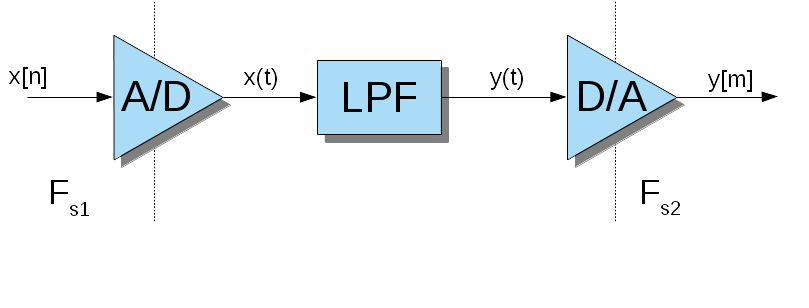
\includegraphics[width=0.8\textwidth]{Figures/classic_analog_alg.png}
  \caption{Analog interpretation of a sample rate converter}
  \label{fig:classic_analog}
\end{figure}

\section{Sample Rate Converter's Structure}
\label{section:asrc_structure}

One of the challenges of creating a purely digital solution is the design of the
LPF digital filter, which is at one time accurate and efficient.  The classical
approach to this problem consists in upsampling the signal by a factor $L$
(interpolation), doing the processing at the frequency $L \times F_{s1}$, and
downsampling the result by a factor $M$ (decimation), as a means to emulate a
discrete to continuous and continuous to discreve signal convertion~\cite{Mitra:HDSP}.
A simple block design of this algorithm is shown in Fig.~\ref{fig:classic_digital}.

\begin{figure}[!htb]
  \centering
  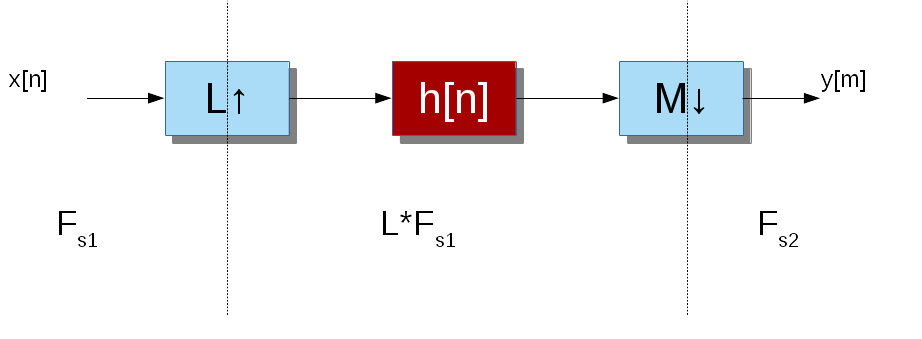
\includegraphics[width=0.8\textwidth]{Figures/classic_digital_alg.png}
  \caption{Classic digital sample rate conversion algorithm by factor L/M}
  \label{fig:classic_digital}
\end{figure}

In practice, an input signal $x[n]$, sampled at frequency $F_{s1}$ is upsampled
by insertion of $L-1$ samples with value zero between two consecutive input samples.
The resultant signal is then inserted into a low pass filter $h[n]$, which will
interpolate the inserted samples and avoid aliasing. Finally, the output of the
filter is downsampled by taking only every $M$-th sample for the output signal
$y[m]$. The relationship between $L$ and $M$ is such that

\begin{equation}
  F_{s2} = \frac{L}{M} F_{s1} .
  \label{eq:FS1_to_FS2_LM}
\end{equation}

Regarding the filter $h[n]$, its cutoff frequency depends on the relationship
described in Equation~(\ref{eq:FS1_to_FS2_LM}).  In the upsampling case ($L \geq
M$), there is the need to remove the resultant spectral images, using a filter
with a normalized cutoff frequency ($\Omega_c \leq 0.5\pi/L$). In the case of
downsampling ($L < M$), there is the need to filter signal frequencies that
would cause aliasing, leading to a filter with a normalized cutoff frequency
($\Omega_c \leq 0.5\pi/M$).  By joining the two conditions, the resultant filter
should have a cutoff frequency

\begin{equation}
  \Omega_c = min(\frac{\pi}{2L}, \frac{\pi}{2M}) [rad] .
  \label{eq:filter_cutoff}
\end{equation}

Note that the normalization considered is in relation to the upsampled frequency:

\begin{equation}
  \Omega = \frac{2\pi f}{Lf_{s1}} [rad].
  \label{eq:freq_norm}
\end{equation}

In the current state of the art, this algorithm is the basis of most synchronous
and asynchronous sample rate converters.

For conversions which use small values of $L$ and $M$ the computational effort is
modest. However, if the conversion involves sampling rates with a small
difference, the factors $L$ and $M$ will increase significantly, increasing
drastically the computational cost of the conversion, only to have most of the
computed samples discarded. Note that in this case a small normalized cutoff
frequency must be used for the filter.

Furthermore, there is the need to design the filter to both remove aliasing and
interpolate the $L-1$ inserted samples. This is why design of the filter $h[n]$
is the main challenge of this architecture. The solution presented in this
thesis is based on the use of a fractional delay filter.

Additionally, for asynchronous sample rate converters, the filter is not
only time-varying, but also varies with the sample rate ratio. This means
that there is the need to define a structure that computes the ratio
and adapts the filter. For synchronous sample rate converters, the ratio
stays constant. This can lead to a predictable filter, leading to the
possibility to trade off storage space for computation time, by
precomputing a finite set of filters~\cite{ad:asrc}.

%%%%%%%%%%%%%%%%%%%%%%%%%%%%%%%%%%%%%%%%%%%%%%%%%%%%%%%%%%%%%%%%%%%%%%%%
\section{Fractional Delay Filter}
\label{section:fd_filter}

An efficient way of obtaining an interpolated value of a sample is to consider
that the output samples needed correspond to the input samples, delayed or
advanced by a certain value. Considering a discrete-time signal $y[n]$, obtained
by delaying a signal $x[n]$,

\begin{equation}
  y[n] = x[n-\tau_d] = x[n] * h_d[n],
  \label{eq:time_delay}
\end{equation}
where $\tau_d$ is the normalized delay. For continuous signals, a time shift in
the frequency domain can be expressed as a product between an input
$X(e^{j\omega})$ and a filter $H(e^{j\omega})$,

\begin{equation}
  Y(e^{j\omega}) = H(e^{j\omega}) X(e^{j\omega}),
  \label{eq:freq_delay}
\end{equation}
where

\begin{equation}
  H(e^{j\omega}) = e^{-j\omega \tau_d}.
  \label{eq:freq_delay_H}
\end{equation}

By analysis of Equation~(\ref{eq:freq_delay_H}), it is possible to note that
a delay filter is an allpass filter with unitary gain and linear phase. However
this is only the case for a continuous time domain $x(t)$ signal. For the
digital signal $x[n]$, which needs to be reconstructed and aliasing-free, a low
pass filter with a cuttoff frequency defined by Equation~(\ref{eq:filter_cutoff})
is needed. Since both the reconstruction and
anti-aliasing filters are linear systems, they can be combined together in a
single filter whose frequency response $H_d(e^{j\Omega})$ is the product of the
frequency responses of the two filters:

\begin{equation}
  H_d(e^{j\Omega}) =   
  \begin{cases}
    1, |\Omega| < \Omega_c \\
    0, otherwise
  \end{cases}
  \label{eq:fdfilter_H}
  .
\end{equation}

To obtain the impulse response of filter $h[n]$, defined in Equation~(\ref{eq:time_delay}),
the inverse discrete-time Fourrier transform (IDTFT) of $H_d(e^{j\omega})$ is
performed.

\begin{equation}
  h[n] = IDTFT(H_d(e^{j\omega})) = \frac{1}{2\pi}\int_{-\pi}^{\pi}e^{-j\Omega\tau_{d}} e^{j\Omega n} d\Omega .
  \label{eq:idtft_h}
\end{equation}

Since the integrated function is non-zero only in the interval $-[-\Omega_c,\Omega_c]$
and $e^{-j\Omega\tau_{d}} e^{j\Omega n} = e^{j\Omega  (n-\tau_{d})}$, the integral can be solved yielding

\begin{equation}
  h[n] = \frac{sin(\Omega_c (n-\tau_{d}))}{\pi (n-\tau_{d})}.
  \label{eq:h_sine}
\end{equation}

The impulse response of the filter $h[n]$ is then defined by Equation~(\ref{eq:ideal_fd}),
which is the normalized $sinc$ function.

\begin{equation}
  h[n] = \frac{\Omega_c}{\pi}sinc\bigg[\frac{\Omega_c}{\pi}(n - \tau_d)\bigg].
  \label{eq:ideal_fd}
\end{equation}

Fig.~\ref{fig:sinc} represents this function for $\tau_{d} = 0$. Note that a
variation of $\tau_{d}$ is equivalent to a translation of the figure in the $n$
(discrete time) axis. By direct observation of the figure, it is possible to
note that for integer values of $\tau_{d}$, $h[n] = 0$ for all samples except
for $n = \tau_{d}$ where $h[n] = 1$. This is the expected filter response for an
integer delay. On the other hand, for a fractional value of $\tau_{d}$, $h[n]$
is non-zero for all samples. For the ASRC algorithm, $0 \leq \tau_{d} \leq 1$,
since the objective is to use this fractional delay filter as a way to obtain an
interpolated sample using a finite number of input neighbour samples separated
by an unitary normalized delay.


\begin{figure}[!htb]
  \centering
  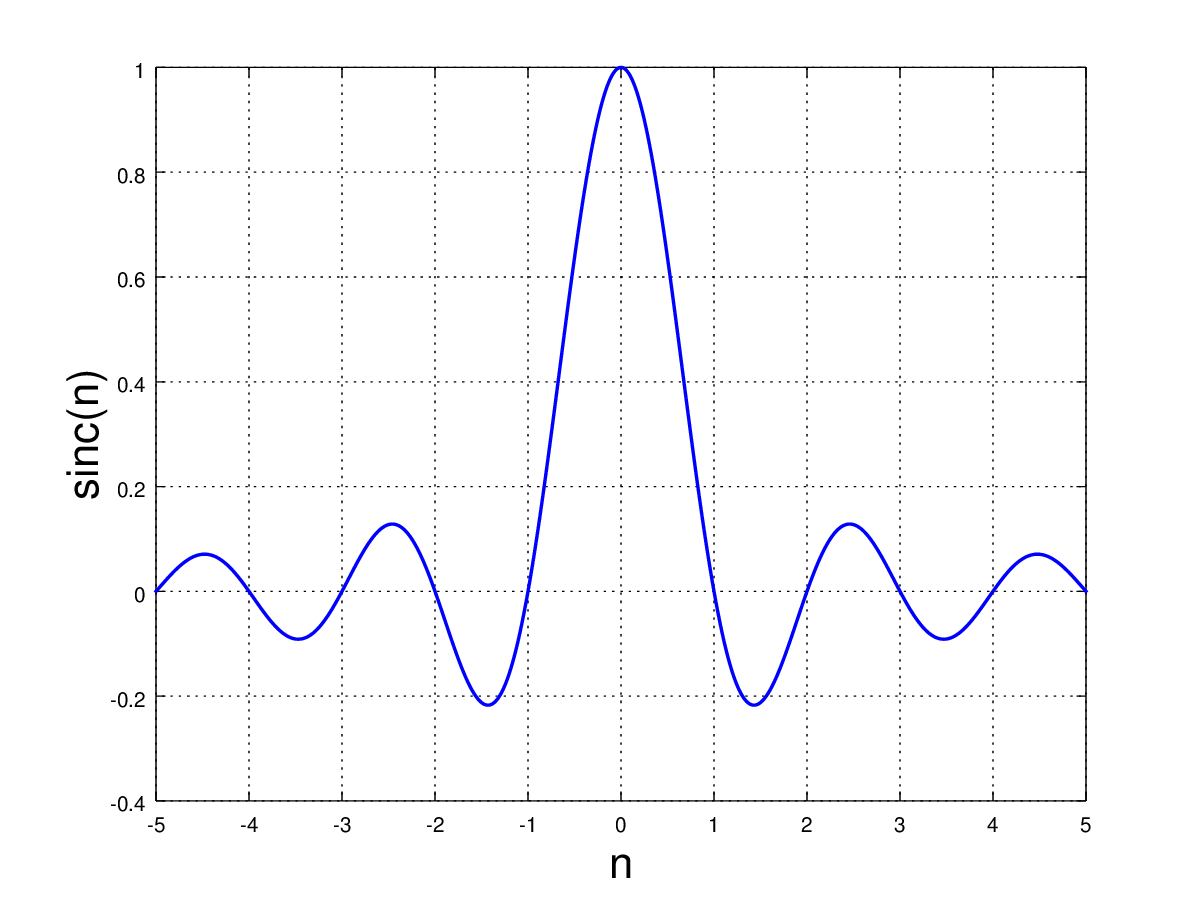
\includegraphics[width=0.8\textwidth]{Figures/sinc.png}
  \caption{Graphical representation of $h[n]$ for $\tau_{d} = 0$}
  \label{fig:sinc}
\end{figure}
  
As this function is infinite and non-causal, an approximation must be done while
retaining enough low-pass filtering capability to ensure quality, as explained
in Section~\ref{section:asrc_structure}. This
problem can be solved by applying a window to the ideal filter $h[n]$. The
choice of the format of the window and bandwidth have an influence not only on
the quality of ASRC's output signal, but also on the complexity of the
computations done.

Using the truncation of the impulse response as an approximation technique, the
resultant filter is a section of the sinc function which contains a certain
number of zeroes. To exemplify, a filter with six zeroes is considered in
Fig.~\ref{fig:exemp_upsamp}, and Fig.~\ref{fig:exemp_downsamp}.

\begin{figure}[!htb]
  \centering
  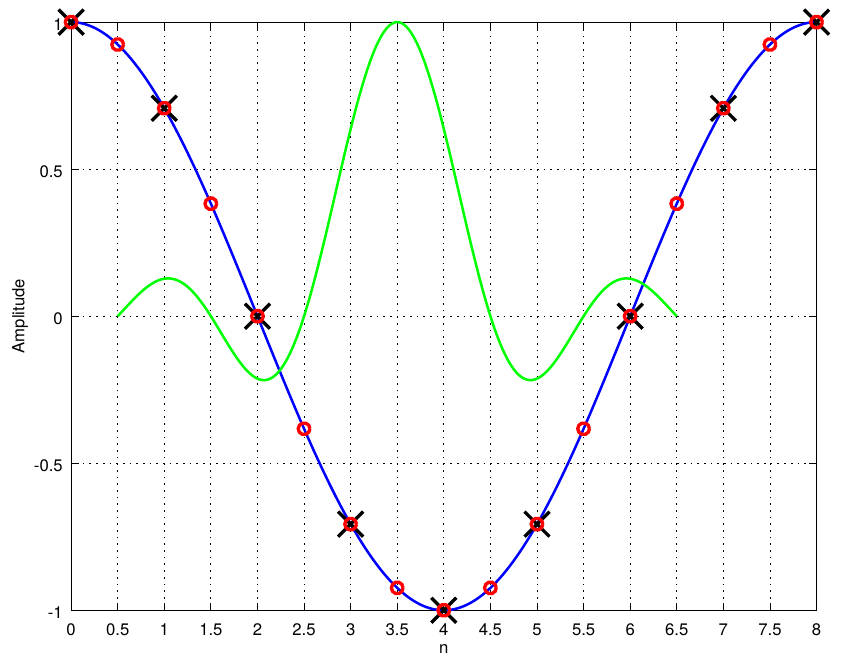
\includegraphics[width=0.8\textwidth]{Figures/upsample_example.png}
  \caption{Illustration of upsampling (1:2) used to determine the output sample
    at n = 3.5}
  \label{fig:exemp_upsamp}
\end{figure}

\begin{figure}[!htb]
  \centering
  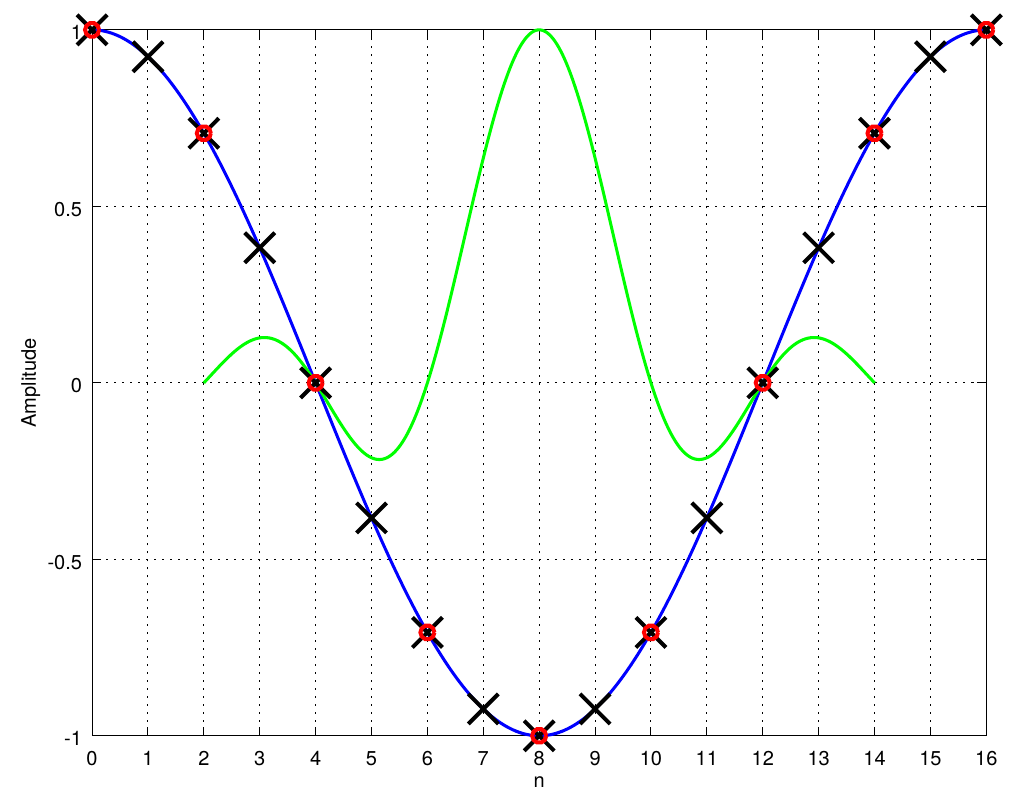
\includegraphics[width=0.8\textwidth]{Figures/downsample_example.png}
  \caption{Illustration of downsampling (2:1) used to determine the output
    sample at n = 4}
  \label{fig:exemp_downsamp}
\end{figure}


In Fig.~\ref{fig:exemp_upsamp}, the digital input signal, whose samples are
represented by crosses, is plotted along its continuous time representation. To
upsample this signal by a factor of 2, the output samples, represented by
circles, need to be computed. To interpolate these signals, the filter
approximation is applied, centring the window at the desired output sample,
multiplying each input sample by the corresponding filter value, and accumulate
all obtained values. By analysis of this illustration, it is possible to note
that a larger upsampling factor will decrease the distance between the output
samples. According to Equation~(\ref{eq:filter_cutoff}), the normalized
cutoff frequency of the filter is $0.5/L$. The filter is always the same in the
upsampling case and its number of accumulations is the same as the number of
zeroes in the truncated sinc function.

Fig.~\ref{fig:exemp_downsamp} is analogous to Fig.~\ref{fig:exemp_upsamp},
representing downsampling by a factor of 2 instead. In this case, according to
Equation~(\ref{eq:filter_cutoff}), the cutoff frequency of the filter is
given by $0.5/M$.  The number of accumulations is now $M$ times the number of
zeroes in the truncated sinc function.

Regarding the approximation of the filter itself, there is a great variety of
techniques used to obtain a fractional delay filter which minimizes the
discretization error: applying a window to the ideal filter, applying Lagrangian
interpolation to compute an intermediate coefficient from a set of known filter
samples, etc. These and other methods are explained in detail
in~\cite{kootsookos:firapproxfd,Tseng:firfdsnr,laakso:pfdfilter,Yardin:Perffdf}.


%%%%%%%%%%%%%%%%%%%%%%%%%%%%%%%%%%%%%%%%%%%%%%%%%%%%%%%%%%%%%%%5
\section{Output Sample Computation}
\label{section:output_computation}

As shown in Fig.~\ref{fig:exemp_upsamp} and \ref{fig:exemp_downsamp}, to obtain
an output sample, the fractional delay filter is applied to the input signal, by
centring it to the desired time of the output sample and computing the result of
the (discrete) convolution, as expressed in Equation~(\ref{eq:time_delay}).
Furthermore, it is important to note that, since this converter is applied to
audio, the digital design of the filter should make sure that the filter has
linear phase. This is achieved by using a Finite Impulse Response (FIR), which
has a non-recursive structure. In an FIR, each output $y[n]$ is obtained by

\begin{equation}
  y[n] = \sum_{i=0}^N a_i x[n-i],
  \label{eq:macc}
\end{equation}

where $a_i$ are the coefficients of the filter and $x[n-i]$ is the input sample
at discrete time $n-i$. It is important to note that the filter described in
Section~\ref{section:fd_filter} is non causal. To fix this, the computation of
the output is delayed by as many input samples as accumulations that involve
future input samples.

With this implementation, the computation of an output sample is reduced to a
multiply-accumulate (macc) operation. However, it requires a large amount of
filter coefficients, which, in hardware, results in high memory usage, an
undesirable result.

To guarantee that the sample rate converter supports multiple
channels, the structure of the converter should be able to support the computation
of multiple output samples. This can be done at the cost of hardware area,
by having one output computation unit per channel, or at the cost of computation
time, by having one unit computing multiple outputs sequentially. To make
this possible, there is the need to optimize this not only regarding hardware
area, but also computation time.

\section{Sample Rate Converter Implementations: An Analysis Of The State Of The Art}
\label{section:implementation}

\subsection{Cascaded Integrator Comb Filters (CIC)}

As was explained in Section~\ref{section:asrc_structure}, sample rate conversion
can be interpreted as signal upsampling with interpolation, followed by
downsampling with decimation. Furthermore, this algorithm can be implemented
using FIR filters as shown in the previous section. One of the designs comonly
used for this purpose is a Cascaded Integrator Comb filter
(CIC)~\cite{charanjit:impl}. This filter, originally designed by Hogenauer~\cite{hogenauer},
is based on the implementation of simple integrators and
differentiators.  CIC filters are obtained by combining adders and delay
registers, which consumes a reduced amount of memory and has the great advantage
of dispensing with multipliers, which can consume a great amount of hardware
resources. Due to the fact that the CIC decimator has a symetric structure in
comparinson to a CIC interpolator, the combination of the two components leads
to a highly efficient implementation in application specific integrated circuits
(ASIC) and FPGA's. An interpolation filter using the CIC structure can be seen
in Fig.~\ref{fig:cic_basic}. A decimation filter would have the same components,
with the difference that the comb filters and integrator stages would swap
positions.

\begin{figure}[!htb]
  \centering
  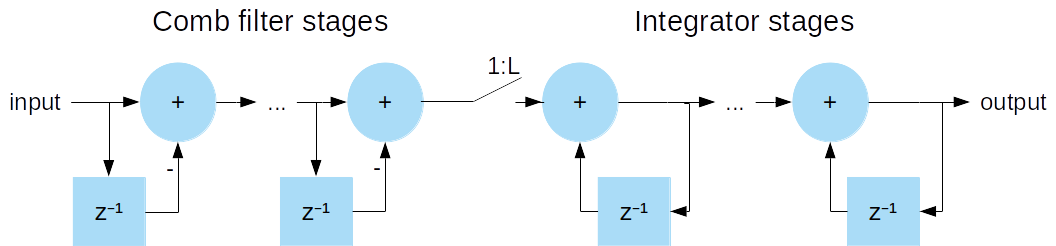
\includegraphics[width=\textwidth]{Figures/cic_filter.png}
  \caption{Example of cascaded integrator comb filter structure, used as an interpolation filter}
  \label{fig:cic_basic}
\end{figure}

While for one CIC structure, the frequency response does not fulfill the
requirements, this problem can be solved by cascating multiple interpolation and
integration units \cite{charanjit:impl}, increasing the attenuation in the
filter's stopband. This implementation is elegant but has limited
configurability, due to the fact that no coefficients are used, making it hard
to adapt the filter to variations in the sample rates. Furthermore, this type of
filter expects integer factors, which leads to the problem of making it able to
convert fractional sample rate relations.

\subsection{Approximation By Piecewise Quadratic Function}
\label{subsection:piecewise}

As explained in Section~\ref{section:fd_filter}, a direct way to implement the
sample rate converter is to consider that the algorithm can be reduced to simply
applying a fractional delay filter to the input signal, with a sinc impulse
response as expressed by Equation~(\ref{eq:ideal_fd}). In practice this is
impossible because the filter has an infinite number of taps and requires the
use of future samples (non-causality).

The solution presented so far is to truncate and approximate the coefficients
and delay the response to make it causal. Another way to address this problem is
to split the sinc function into a piecewise function, and aproximate each piece
by a quadractic function, leading to an interpolation filter which can be easily
implemented~\cite{aikawa:kernel,aikawa:kernel_hw}. The approximation of the
piecewise sinc function $h(x)$ into quadractic functions can be expressed as

\begin{equation}
	h(t) = 
	\begin{cases}
		a_{1,1}t^2+b_{1,1}t + c_{1,1}, \bigg(0 \leq |t| \leq \frac{1}{N}\bigg)\\
		\vdots \\
		a_{1,n}t^2+b_{1,n}t + c_{1,n}, \bigg(\frac{n-1}{N} \leq |t| \leq 1\bigg)\\
		\vdots \\
		a_{s,n}t^2+b_{s,n}t + c_{s,n}, \bigg(s-1+\frac{n-1}{N} \leq |t| \leq s-1+\frac{n}{N}\bigg)\\
		\vdots \\
		a_{S,n}t^2+b_{S,n}t + c_{S,n}, \bigg(S-1+\frac{n-1}{N} \leq |t| \leq S\bigg)
	\end{cases}
,
	\label{eq:kernel}
\end{equation}
where $N$ is the number of quadratic functions used to represent a piecewise
function, and $S$ is the number of piecewise functions of the kernel. This
technique leads to the implementation presented in Fig. \ref{fig:kernel}.

\begin{figure}[!htb]
  \centering
  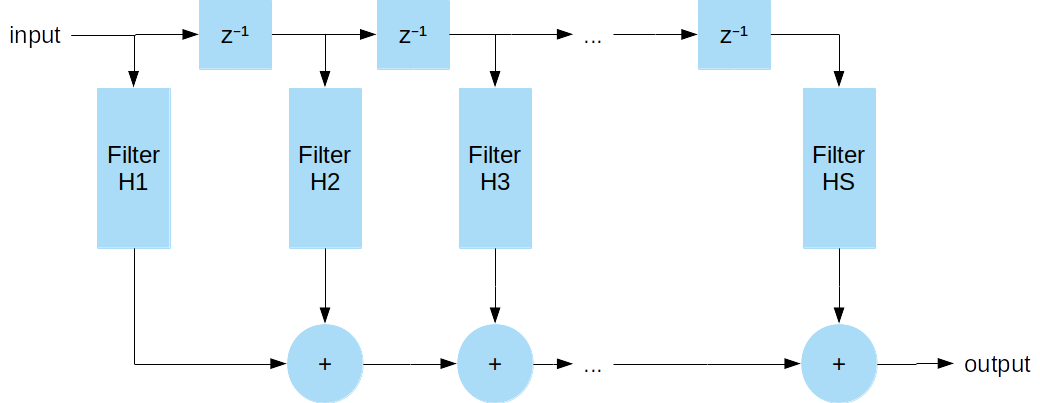
\includegraphics[width=\textwidth]{Figures/kernel_filter.png}
  \caption{Example of a piecewise kernel filter structure}
  \label{fig:kernel}
\end{figure}

This design can be futher optimized, by considering that from a certain section
onward, the polynomial remains the same, changing only in scale by a determined
set of factors $e_j$. The block diagram of this structure is presented in
Fig.~\ref{fig:kernel_block}. This leads to a structure where the polynomials
used remain the same, while the factors $e_j$ change with the sample rate
convertion ratio. There are, however, some restrictions that need to be
considered, as further explained in~\cite{aikawa:kernel}.

\begin{figure}[!htb]
  \centering
  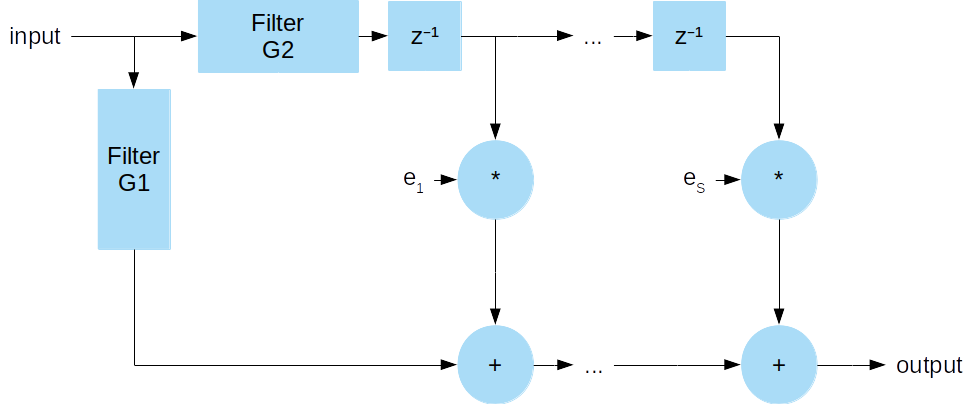
\includegraphics[width=\textwidth]{Figures/kernel_filter_2.png}
  \caption{Example of optimized kernel filter structure}
  \label{fig:kernel_block}
\end{figure}

The main advantage of this design is the ability to change sample rate ratio
without need to reconfigure the filter, leading to a kernel which not only is
able to implement the function, but also does not need to change over
time. However, as one needs to define a high number of pieces to obtain large
attenuation in the stopband (to acceptably attenuate distortion and noise), it
is needed to use a large number of quadratic functions, which significantly
increases the computational cost. Apart from the structure itself, there is
still the high cost of computing the coefficients $e_j$, which turns even more
problematic with applications for which the sample rate convertion ratio varies
in time.

\subsection{Farrow Structure}

The most common implementations of fractional delay filters, and, by
consequence, sample rate converters, is one which uses the Farrow Structure
\cite{Farrow:farrow_structure}.  This structure is based on the assumption that
each sample of the filter impulse response $h[n]$ can be approximated by a
polynomial of order $q$, which depends on the fractional delay
$d$~\cite{Blok:VariableRS}:

\begin{equation}
	h[n] = \sum_{m=0}^{q} c_m[n]d^m.
	\label{eq:farrow_approx}
\end{equation}

Similar to the structure presented in Section~\ref{subsection:piecewise}, a
Farrow structure requires the implementation of a set of $q$ FIR filters, which
becomes a hardware-intensive design. Furthermore, a change in the fractional
delay forces the change of all coefficients, leading to an increase of the
computational cost. Over the years, this structure has been subjected to many
changes and optimizations, with the objective to develop filters for different
applications. For the specific application this thesis is concerned, the
structure is optimized to design filters with a variable fractional delay.  One
possible optimization, further explained in~\cite{babic:farrow_optimization},
makes it possible to implement a low area Farrow structure, with the great
advantage of having fixed coefficients and a single parameter $\mu$ that depends
on the fractional delay. The block design of this structure is presented in
Fig.~\ref{fig:farrow_structure}, where the value of $\mu$ can be computed by

\begin{figure}[!htb]
  \centering
  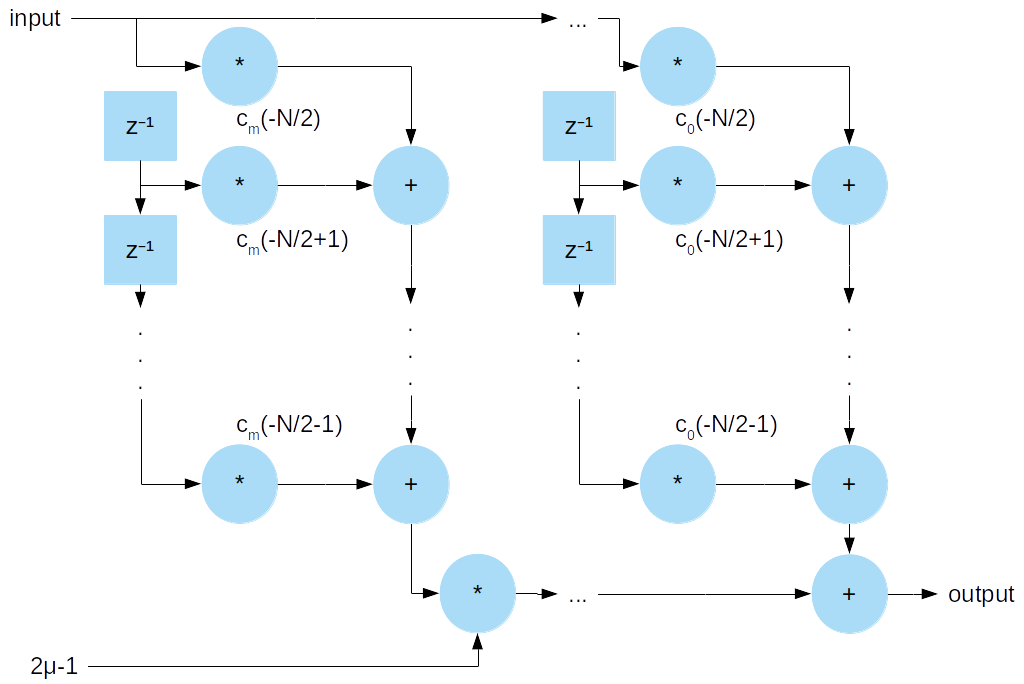
\includegraphics[width=\textwidth]{Figures/farrow_struct.png}
  \caption{Example of farrow structure, optimized for variable fractinal delay}
  \label{fig:farrow_structure}
\end{figure}


\begin{equation}
	\mu = \frac{k}{M},
	\label{eq:mu_farrow}
\end{equation}
where $M$ is the decimation factor and $k \in \{0,1,2,...\}$, is a value which
increments throughout the computation of the output. The transfer function of
each FIR subfilter, $C_m (z)$ is expressed by

\begin{equation}
	C_m (z) = \sum_{k=0}^{N-1}c_m \bigg(k-\frac{N}{2}\bigg)z^{-k} .
	\label{eq:farrow_sub_transferfunc}
\end{equation}

While the structure presented in Fig.~\ref{fig:farrow_structure} is optimized
for interpolation, there are some modifications, explained in detail
in~\cite{babic:farrow_optimization} which apply to decimation. This structure has
the disadvantage of having to include all subfilters to compute all coefficients
$c_n$, it is one of the easiest methods to allow variations on sample rate
conversion ratios, and occupies a low area, which is mainly taken by the delay
elements.
 % file "Thesis_ASRC.tex"
\cleardoublepage

\chapter{Circuit Design}
\label{chapter:circ_design}

The symbol and interface signals of the sample rate converter design is
presented in Fig.~\ref{fig:bd_top_iface}. The data input and output signals are
$x$ and $y$, respectively, and the sample rate clocks are $x\_clk$ and $y\_clk$,
respectively. The definition of all interface signals is presented in
Table~\ref{tab:top_iface}.

\begin{figure}[!htb]
  \centering
  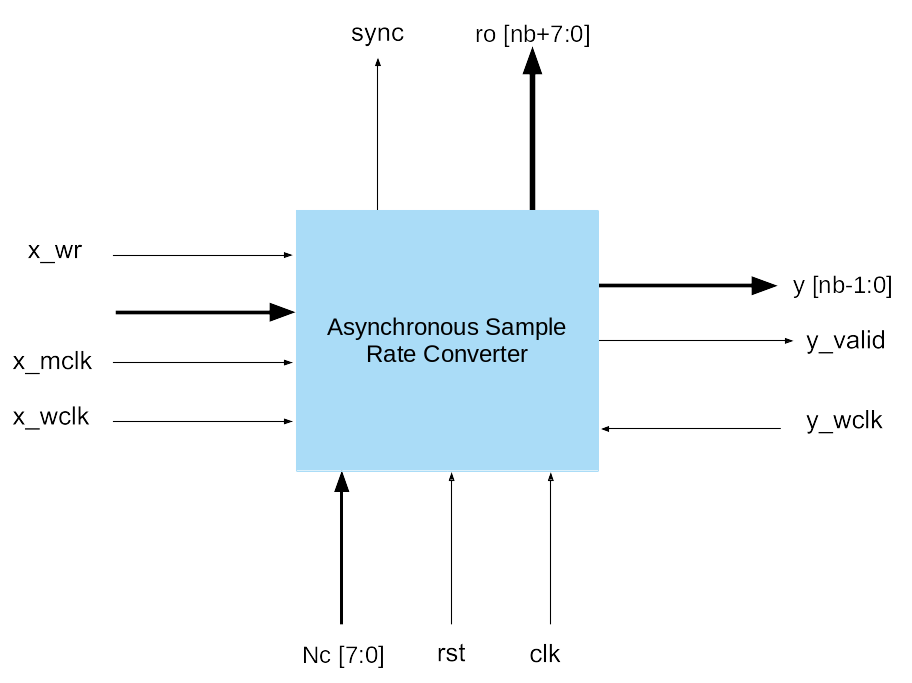
\includegraphics[width=0.7\textwidth]{Figures/asrc_iface_bd.png}
  \caption{Asynchronous sample rate converter interfaces block diagram.}
  \label{fig:bd_top_iface}
\end{figure}

\begin{table}[!htbp]
  \centering
  \caption{List of asynchronous sample rate converter interface signals.}
  \label{tab:top_iface}
  \begin{tabular}{|c|c|p{0.7\linewidth}|}
    \hline 
	{\bf Name} & {\bf Direction} & {\bf Description} \\ \hline
        \hline
	clk & Input & System clock input.\\ \hline
	rst & Input & Active high synchronous reset.\\ \hline
        \hline
        Nc [7:0] & Input & Number of input audio channels.\\ \hline
        \hline
        x [nb-1:0] & Input & Input sample.\\ \hline
        x\_wclk & Input & Input word clock, with frequency equal to the input sample rate.\\ \hline
        x\_mclk & Input & Input master clock. Should be $2^N$ times faster than x\_wclk, where N is an integer
        greater than Nc.\\ \hline
        x\_wr & Input & Input sample write enable.\\ \hline
        \hline
        y [nb-1:0] & Output & Output sample.\\ \hline
        y\_wclk & Input & Output word clock, with frequency equal to the output sample rate.\\ \hline
        y\_valid & Output & Output sample valid. Should be used as an enable to an output
        sample register.\\ \hline
        \hline
        ro [nb+7:0] & Output & Sample rate convertion ratio signal. Represented in format
        8Qnb.\\ \hline
        sync & Output & Active high when the converter has stabilized.\\ \hline
  \end{tabular}
\end{table}

The ASRC is divided in three modules: the Input Data Memory, the Ratio Estimator
and the Resampler. Additionally, a simple positive edge detector circuit is
needed to start the execution of some modules. A block diagram of the
ASRC with its three modules is presented in Fig.~\ref{fig:bd_top}.

The core works in three different clock domains and all figures present the
signals in three different colors, with green arrows indicating signals in
$x\_mclk$'s domain, blue arrows for signals in $y\_wclk$'s domain, and black
arrows for signals in $clk$'s domain. This is important as wherever there is a
clock domain crossing there needs to be a suitable synchronizer circuit.

\begin{figure}[!htb]
  \centering
  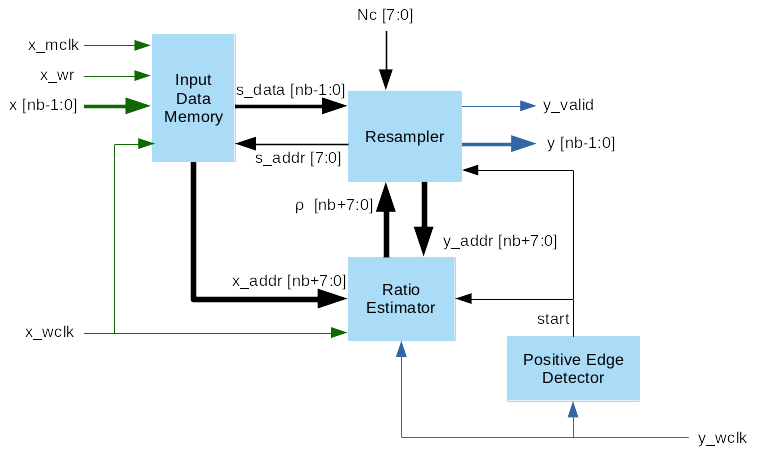
\includegraphics[width=0.8\textwidth]{Figures/asrc_top_bd.png}
  \caption{Asynchronous sample rate converter top block diagram.}
  \label{fig:bd_top}
\end{figure}

\section{Data Memory}
\label{section:data_mem}

To store the input samples, a data memory is used. This data memory should be a
dual port Random Acess Memory (RAM) capable of working at two different clock
domains. The block diagram of this memory and the auxiliary components to access
is presented in Fig.~\ref{fig:bd_datamem}.

\begin{figure}[!htb]
  \centering
  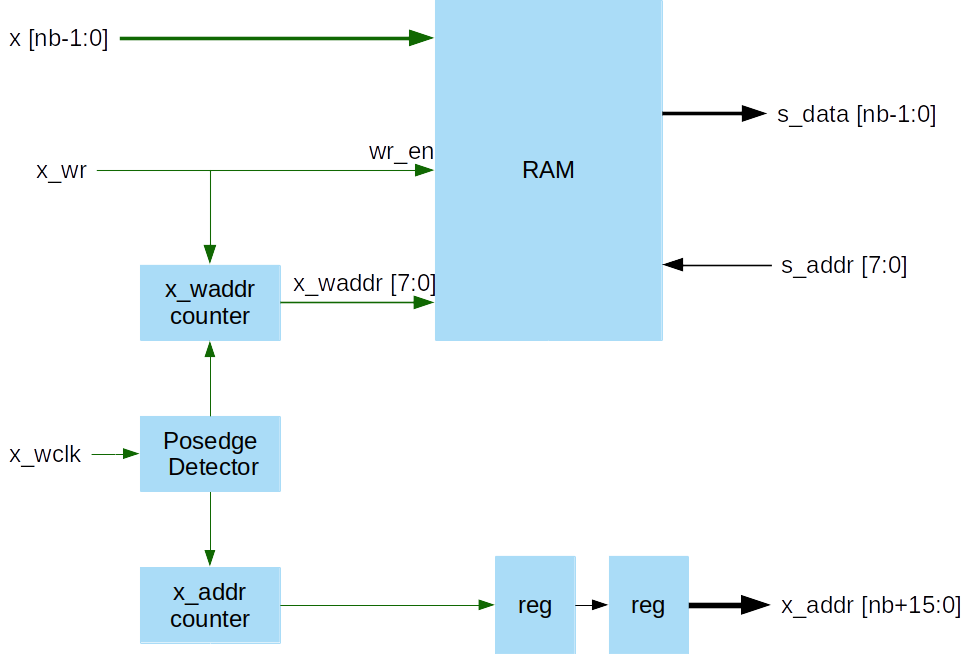
\includegraphics[width=0.8\textwidth]{Figures/asrc_datamem_bd.png}
  \caption{Data memory module block diagram.}
  \label{fig:bd_datamem}
\end{figure}

In the input clock domain, the samples $x$ are stored in the position given by
$x\_waddr$ at the rate of $x\_mclk$. The write address counter $x\_waddr$ is
incremented at $x\_mclk$'s rate, whenever $x\_wr$ is active.
In the time domain of the system clock, the
samples are read by accessing the position given by $s\_addr$. For each output
clock pulse, the input samples needed to perform the filtering are read from the
memory at the system clock rate. For a multiple channel input, to obtain the
next sample of a certain channel, the address $s\_addr[n+1]$ is given by
\begin{equation}
  s\_addr[n+1] = s\_addr+Nc.
  \label{eq:datamem_nextsample}
\end{equation}

Since the accumulators do not stop or reset during the execution of the
conversion, they wrap around creating a circular memory. When there is a stream
of input samples, the newer ones will overwrite the older ones which will not be
used anymore in the time-finite fractional delay filter.  On average the write
and read pointers increment at the same rate, which is guaranteed by the Ratio
Estimator block.

This module also contains an additional counter, $x\_addr$. This counter
is similar to the $x\_waddr$ counter, with the difference that it is
not controlled by $x\_wr$. This counter is used by the ratio estimator
described in Section~\ref{section:ratio_est}, as an parameter used
to adjust the sample rate conversion ratio.


\section{Ratio Estimator}
\label{section:ratio_est}

Since the sample rate converter is asynchronous, the frequency of the input and
output clocks can change over time. Furthermore, their frequencies can also take
any value in the supported range. The frequencies of the data clocks are unknown
by the core but their ratio must be computed. The Ratio Estimator is the module
that computes the ratio between the periods of the data clocks, and its block
diagram is shown in Fig.~\ref{fig:bd_ratioest}.

\begin{figure}[!htb]
  \centering
  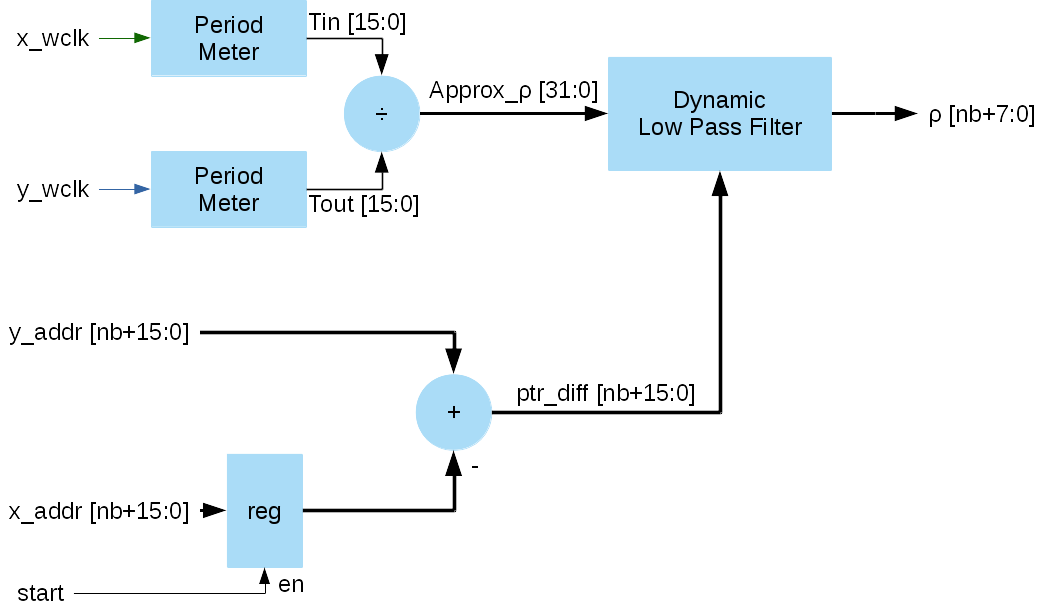
\includegraphics[width=0.8\textwidth]{Figures/asrc_ratioest_bd.png}
  \caption{Ratio Estimator module block diagram.}
  \label{fig:bd_ratioest}
\end{figure}


The Period Meter block uses a counter to obtain a relative value $T_{count}$ of
the period of the data clocks. Since the counter is incremented at the system
clock rate $f_{sys\_clk}$, an approximate value of the data clock period $T_d$
is given by

\begin{equation}
  T_d = \frac{T_{count}}{f_{sys\_clk}}.
  \label{eq:samp_rate_period}
\end{equation}

The ratio $\rho$ between the input and output clock frequencies $f_{in}$ and $f_{out}$
is defined by

\begin{equation}
  \rho = \frac{f_{out}}{f_{in}}.
  \label{eq:rho_teo}
\end{equation}

Combining Equation~(\ref{eq:samp_rate_period}) and~(\ref{eq:rho_teo}), an
approximate value of $\rho$ can be computed by

\begin{equation}
  \rho  = \frac{T_{count\_in}}{T_{count\_out}}.
  \label{eq:rho_hw}
\end{equation}

The value of $\rho$ can be computed in hardware without knowing any clock
frequencies. However, since the counter is only able to count integer values,
the periods of the input and output clocks are imprecise.  For the same clock
frequency the value $T_{count}$ can vary each time it is determined, with an
absolute error of 1 unit. It should be noted that the resolution of the counter
increases with the frequency of the system clock: a higher system clock
frequency leads to a lower error in $T_d$.

These errors lead to an imprecise value of $\rho$, leading not only to an error
in the conversion done in the resampler module, but also to having the read and
write pointers in the data memory module incrementing at different average
speeds, which eventually may cause the buffer to underflow or overflow. The
dynamic low pass filter is the block which solves this problem, as it stabilizes
the deviations of the approximate result of $\rho$, obtained according to
Equation~(\ref{eq:rho_hw}), obtaining the mean value instead. The structure of
the dynamic low pass filter is not given at this stage. It will simply be stated
that when there is a high deviation of the approximate $\rho$, the filter's
cuttoff frequency rises, as it assumes there was a change of the input and/or
output clock frequencies. When the deviation lowers, the filter's cuttoff
frequency lowers as well, being less sensitive to the small deviations of the
approximate $\rho$ caused by quantization and period counting errors. A
correction parameter that takes into account the difference between the read and
write pointers of the input data memory adjusts the value of $\rho$. The read
pointer increment rate is changed to keep the difference between the pointers
constant, for example, ensuring that the read and write pointers have a distance
equal to half of the memory's size.


\section{Resampler}
\label{section:resampler}

The resampler is the main module of the sample rate converter and executes the
conversion algorithm. This complex module is split into three submodules: the
\textit{address generator}, the \textit{coefficient memory} and the
\textit{multiply-accumulate} submodule, which are explained in the next
subsections. A block diagram of the resampler is presented in
Fig.~\ref{fig:bd_resampler}.

\begin{figure}[!htb]
  \centering
  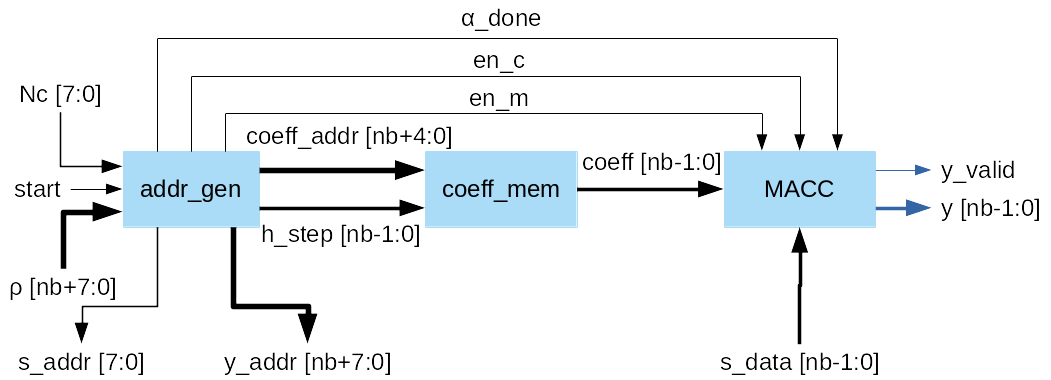
\includegraphics[width=0.8\textwidth]{Figures/asrc_resampler_bd.png}
  \caption{Resampler module block diagram.}
  \label{fig:bd_resampler}
\end{figure}

\subsection{Address Generator}
\label{subsection:addr_gen}

The address generator is the submodule responsible for computing the addresses
of the input samples needed to compute the output sample. As explained in
Sections~\ref{section:fd_filter} and~\ref{section:output_computation}, there
are two main steps needed to compute an output sample: (1) center the filter at
the time of output sample to be computed; (2) compute the input samples and
correspondent filter coefficients and perform the filter convolution operation.

To center the filter at the time of the output sample to be computed, an alpha
computation submodule is used. This submodule computes the time of the current
output sample to be computed in the form of a fractional address $y\_addr$,
which is incremented by a factor $1/\rho$ at the output sample rate.

Additionally, there is the need to know the distance in time (normalized to the
input's sample rate) between the current output sample and the closest input
sample, as this distance defines the first coefficient to be used for each side
of the symmetric filter. This distance is called $\alpha$ and is computed by
assuming that there is an input sample $x[n]$ for all integer values of $n$, and
that $1-\alpha$ is the fractional distance between the output sample and the
closest input sample.

Finally, to adapt the filter's shape, ensuring that it has a cutoff frequency
defined by Equation~(\ref{eq:filter_cutoff}), a parameter $h\_step$ is defined
by normalizing the cutoff frequecy to the input sample clock frequency:

\begin{equation}
  h\_step = min(1, \rho).
  \label{eq:h_step}
\end{equation}

With the value of $h\_step$ and $\alpha$, as well as the integer part of
$y\_addr$, it is possible to determine all of the needed addresses for the input
samples and correspondent coefficients.

To get the input samples' addresses a simple counter submodule
(\textit{s\_addr  computation}) is used.
The integer part of $y\_addr$ is used as the base of the address computation.
Knowing that consecutive input samples of the same channel have the distance defined by
Equation~(\ref{eq:datamem_nextsample}), it suffices to accumulate this distance
from the offset of the current channel to get all needed input sample addresses
that come after (or to the right of) the output sample instant. When the right
side is completed, the left side is computed by negative accumulations from the
channel offset, getting the addresses of all input samples before the output
sample instant. When both sides are done, the channel offset is incremented and
the process is repeated for the next channel. This means that one channel is
computed at a time, allowing the use of a single multiply-accumulate unit to
compute the output samples for all channels.


To get the coefficients' addresses, another accumulator is used. The value of
$\alpha$ is used as the initial value in order to align the input sample to its
filter coefficient. Since an increment of one input sample corresponds to a
increment of $h\_step$ in the coefficient function, $h\_step$ is used as the
accumulation value. These accumulations will be done until the filter is no
longer defined, which happens when the accumulator reaches or overcomes the
final address of the coefficients memory. After these accumulations are done,
there is a side switch, and the accumulations restart, with the complement
$1-\alpha$ as the initial value and the same increment of $h\_step$. This module
also produces two flags, $en\_m$ and $en\_c$, to enable accumulations and reset
the accumulator when the channel is done, respectively.

\subsection{Coefficient Memory}
\label{subsection:coeff_mem}

To get the filter's coefficients, the simplest way is to have a lookup table
with them already pre-computed using a Read Only Memory (ROM).  Because
of the high precision needed the ROM would be too large.  To solve this problem,
a simple linear interpolator is used. Assuming that a certain coefficient
$h[i+\Delta]$ is needed, $h[i]$ and $h[i+1]$ exist in the lookup table, and
$\Delta$ is a fractional positive distance to $i$, the coefficient is obtained
by

\begin{equation}
  h[i+\Delta] = h[i] + \Delta (h[i+1]-h[i]).
  \label{eq:coeff_interpol}
\end{equation}

\subsection{Multiply-Accumulator}
\label{subsection:macc}

This submodule is a simple accumulator, done with a register and an adder. Its
input is the product between the coefficient and the input sample as defined by
Equation~(\ref{eq:macc}). Its initial value is set by directly loading (not
accumulating) the first product.

The final register, which produces the output $y$, is enabled only when all
accumulations have finished. This ensures that $y$ never has an intermediate
value. This output is updated at the output sample rate but lives in the system
clock domain. Therefore a synchronizer is further needed to convert it to the
$y\_wclk$ clock domain.
 % file "Thesis_Design.tex"
\cleardoublepage

%%%%%%%%%%%%%%%%%%%%%%%%%%%%%%%%%%%%%%%%%%%%%%%%%%%%%%%%%%%%%%%%%%%%%%%%
%                                                                      %
%     File: Thesis_Results.tex                                         %
%     Tex Master: Thesis.tex                                           %
%                                                                      %
%     Author: Gonçalo Santos                                           %
%     Last modified : 20 Oct 2018                                      %
%                                                                      %
%%%%%%%%%%%%%%%%%%%%%%%%%%%%%%%%%%%%%%%%%%%%%%%%%%%%%%%%%%%%%%%%%%%%%%%%

\chapter{Results}
\label{chapter:results}

The aim of this work is to produce a workable {\bf C} language
compiler for the {\it Versat} architecture using the {\it picoVersat}
instruction set.
The success can be measured by the number of {\bf C} language
constructs that are working properly.
Consequently, testing is of primordial importance, as are the range
of tests used to exercise the compiler.

\section{Functionality}

The compiler, as far the tests were comprehensive,
supports all {\bf C} language integer constructs.
Limitations are listed below.

Since the processor instruction set is reduced, as are the
number of {\bf lcc} terminals to be implemented by the compiler,
the testing of each operation, on its own, is strait
forward.
Testing sequences of such operations may prove more
difficult to test, since different {\bf C} programs
can produce different selection matches.

\section{Testing}

In the test of a compiler, where a small change can affect the
generation of multiple instructions, a good set of
regressive tests is very important.
In order to automate the process, a {\tt test/} directory
was setup.
This directory includes a set of {\bf .c} test files and
the expected output {\bf .out}.

The {\tt Makefile} compiles, executes and compares the new
result with the previously stored result.
All differences in output are printed and can then be analyzed.

Since the output from {\bf iverilog} includes the number
of clocks spent, it is easy to compare whether the changes in the
compiler result in improvements, or in performance degradation.

Some tests are very simple and its output can be easily predicted.
To make testing even simpler, the return value of the {\tt main}
routine is printed, unless the {\sc NORET} environment variables
is defined. Upon return from the {\tt main} routine, the lowest
nibble is printed as an {\sc ASCII} starting at $0$.
This means that values between $10$ and $15$ are printed as
the {\sc ASCII} character at the respective offset, namely the
sequence: \verb|:|, \verb|;|, \verb|<|, \verb|=|, \verb|>|, \verb|?|.

More complex tests can be compiled with {\bf gcc} and executed
to access the expected output.
This, however, can not be performed if the examples include
{\tt asm} calls, since the code can only be executed by the
{\it Versat}, or by the {\bf iverilog} simulator, and not by the
native testbench processor.
%vdb.c

A set of $86$ regression tests is currently being used, ranging
from specific operator testing to complex recursive and iterative
examples. % And the number of tests keeps growing ...

\section{Limitations}\label{limitations}

The {\bf C} language imposes that {\tt sizeof(char)==1}
as does the {\bf lcc} compiler (see~\cite[p.79]{hanson95}).
This works fine as far as {\tt sizeof(char)} can be 32-bits.
However, additionally, the {\bf lcc} assumes through out
the code that $8$ is the number of {\em bit-per-byte}.
If it was a variable, one could set it to $32$.
As it is hardcoded, all address literals
will be truncated to 8-bits ({\tt 8}${}^{\wedge}${\tt ty->size}).
\begin{verbatim}
int *addr = (int*)0x123456;
\end{verbatim}
This can be avoided by setting an integer to the
required value and then assigning it to a pointer.
This works since integer literals are 32-bit wide
and the conversion to pointer, controlled by the
{\it back-end}, does not truncate the value.
\begin{verbatim}
int *addr, value = 0x123456;
addr = (int*)value;
\end{verbatim}
Nevertheless, defining literal pointer is never
a good predictive in virtual memory machines.
In {\it Versat} it is useful to map variables
to specific addresses.

Due to the same reason, a warning message is issued
({\tt shifting an `int' by 12 bits is undefined})
but the code is correctly generated.

% #define LONG_MIN -2147483648
% warning: unsigned operand of unary -
% but 0x80000000 or bellow is OK!
% #  define LONG_MAX	2147483647
% #  define LONG_MIN	(-LONG_MAX - 1L)

In the initial version of {\it picoVersat}, all global
data must be added by {\tt MEM\_BASE=512}.
Since this is performed when addresses are fetched,
static assignments store the unadded value.
Therefore, all accesses must be added by $512$.
Must add {\tt 512} to global pointers in {\tt picoversat-0.0}
\begin{verbatim}
int mem[10], *base = mem;
int main() { base[6+512] = 9; return return mem[6]; }
\end{verbatim}
This can be avoided if assignment is performed during
execution (not at compile time), even if the variable
is global.
\begin{verbatim}
int mem[10];
int main() { int *base = mem; base[6] = 9; return return mem[6]; }
\end{verbatim}

Signed multiplication, division and modulus ({\tt \_mul},
{\tt \_div} and {\tt \_mod}) do not generate carry since
the flags register of {\it picoVersat} is read-only.

The {\bf C} programming languages relies on separate
compilation, where several files are independently
compiled and then linked together.
However, there is no linker in the {\it Versat} system
and the assembler {\bf va} does not support multiple
files.
The solution is to perform linking with {\bf cpp} %%%
include directives.
While in normal {\bf C} the {\tt .c} should be
included, rather compiled, the inclusion of {\bf .h}
as well as {\bf .c} accomplishes the desired result.
Since there is no linking, only multiple inclusion
of files must be avoided.

The {\it Versat} architecture is meant to be used offline
and no form of argument passing to the {\tt main} routine
is available.
Consequently, the stack is initialized at the top.
Therefor, even if the program declares arguments to
the {\tt main} routine ({\tt argc, argv, envp}) they should
never be accessed.
Also, since the system has no memory management unit,
all illegal accesses are silently ignored by the system.
Highly recursive routines that exhaust the stack will have
unpredictable behaviors, since they will begin to overwrite
the top of the code.
Even if it is not the compilers responsibility, it something
that the programmer should be aware, especially when
transitioning from a virtual managed memory system.

Finally, the compiler does not support floating point
data types, since every operation must be supported
by library routines.
This is the case for many android devices, namely
smartphones.
However, the {\it Versat} purpose is to perform
integer arithmetic operations fast and is not aimed at
scientific programming.
The error message {\tt compiler error in \_label--Bad terminal}
is issued by the compiler when it cannot handle a given operation,
namely floating point operations.

\section{Register assignment}

Register assignment in compiler design considers two types of registers:
global registers that hold variable values and scratch registers that hold
temporary values.
The {\bf lcc} compiler defines these registers by setting a mask for each
type of register.
It is up to each {\it back-end} to define the mask values according to processor
capabilities.
For instance, the {\bf sparc} processor defines $4$ sets of $8$ registers:
global, temporary, input and output; where the later two sets replace
the stack for argument passing.
In {\bf i386} all $7$ registers are temporary, while {\bf mips} uses half
for each purpose ($16+16$).

Since the {\it picoVersat} has no specific register assignment, a study
was carried out in order to assess the best balance between global and
scratch registers.
Registers {\tt R0} and {\tt R13} to {\tt R15} are used to communicate with {\it Versat}
and are invisible to the compiler.
The stack is controlled by a {\it stack pointer} ({\tt R12}) and a {\it frame pointer}
({\tt R11}).
The remaining registers ({\tt R1} to {\tt R10}) compose a mask {\tt 7FE}, where
the lowest bit ({\tt R0}) is omitted for register assignment, and the highest
used bit {\tt 400} is {\tt R10}.
The register {\tt R1} is used to return function values and all arguments are
passed on the stack.
At least two registers must be used as scratch for binary operations
temporaries.
The compiler allows the definition of a {\tt tmask} for temporaries and a
{\tt vmask} for variables.

Initially, in run $1$, the experiment uses all registers for temporaries.
Each run adds a variable register at the expense of a temporary, until only
two temporaries remain (run $9$).
Three examples where used: {\tt assign}, {\tt repeating locals} and
{\tt bubble sort}.
The first two represent opposite extremes of register usage, while the last is
a more balanced and realistic example.

The first example uses the {\bf C} language right associative {\it assign} operator
where each new assignment to the variable {\tt a} requires a new temporary register.
%(see Figure~\ref{fig:assign}).

%\begin{figure}
\begin{verbatim}
int f() { return 1; }
int main()
{
  int a;

  a = f() + (a =
      f() + (a =
      f() + (a =
      f() + (a =
      f() + (a =
      f() + (a =
      f() + (a =
      f() + (a =
      f() + (a =
      f() + (a =
      f() + (a =
      f() + (a =
      f() + (a = 1
                  )))))))))))));
  return a;
}
\end{verbatim}
%\caption{}
%\end{figure}

The register usage shows that each assign uses a register $4$ times at
the expense of the return register {\tt R1}.
The best solution, represented by the lowest clock count,
is to use only two temporaries, since more variables imply more stack ({\tt R12}),
saves and restores between each call to the function {\bf f}.

%\begin{table}
\begin{center}
{\small
\begin{tabular}{r|r|r|r|r|r|r|r|r|r|r|r|r|r|r|r|r}
run&vars&vmask&tmask&R1&R2&R3&R4&R5&R6&R7&R8&R9&R10&R11&R12&clks\\\hline
1&0&000&7FE&21&4&4&4&4&4&4&4&6&44&27&82&677\\
2&1&400&3FE&23&4&4&4&4&4&4&6&42&17&14&82&638\\
3&2&600&1FE&25&4&4&4&4&4&6&42&0&17&16&77&633\\
4&3&700&0FE&27&4&4&4&4&6&42&0&0&17&18&72&628\\
5&4&780&07E&29&4&4&4&6&42&0&0&0&17&20&67&623\\
6&5&7C0&03E&31&4&4&6&42&0&0&0&0&17&22&62&618\\
7&6&7E0&01E&33&4&6&42&0&0&0&0&0&17&24&57&613\\
8&7&7F0&00E&35&6&42&0&0&0&0&0&0&17&26&52&608\\
9&8&7F8&006&39&42&0&0&0&0&0&0&0&17&28&47&603\\
\end{tabular}
}
\end{center}
%\caption{}
%\end{table}
\vspace*{5mm}

The second example uses lots of repeating local variables so that each one is assigned
a register, for its uses from the first to last line, if one is available.
%(see Figure~\ref{fig:locals}).

%\begin{figure}
\begin{verbatim}
int func(int a, int b, int c, int d, int e, int f, int g, int h, int i, int j, int k) {
    a = a + b - c - d - e + f - g + h + i + j + k;
    b = a - b + c + d - e - f + g - h + i - j - k;
    c = a + b - c - d + e + f + g - h + i + j - k;
    d = a - b - c + d - e + f - g + h - i - j - k;
    e = a + b + c - d - e - f - g + h - i + j - k;
    f = a - b - c + d - e + f + g - h - i - j + k;
    g = a + b - c - d + e + f + g - h + i + j - k;
    h = a - b + c + d - e - f - g + h + i - j - k;
    i = a + b - c - d - e + f + g + h + i + j - k;
    j = a - b - c + d - e + f + g - h - i - j - k;
    k = a + b + c - d + e - f - g - h - i + j + k;
    return a + b + c + d + e + f - g + h - i + j - k;
}

int main() {
    return func(10, 9, 8, 7, 6, 5, 4, 3, 2, 1, 0);
}
\end{verbatim}
%\caption{}
%\end{figure}

As expected, the best solution is to use highest of temporaries in order
to reduce frame pointer ({\tt R11}) accesses to stack saved values.

%\begin{table}
\begin{center}
{\small
\begin{tabular}{r|r|r|r|r|r|r|r|r|r|r|r|r|r|r|r|r}
run&vars&vmask&tmask&R1&R2&R3&R4&R5&R6&R7&R8&R9&R10&R11&R12&clks\\\hline
1&0&000&7FE&45&27&12&13&48&46&40&45&54&62&68&56&956\\
2&1&400&3FE&53&31&13&54&46&40&47&54&62&0&78&51&1001\\
3&2&600&1FE&61&35&52&46&48&49&56&62&0&0&89&46&1051\\
4&3&700&0FE&89&39&59&63&51&56&62&0&0&0&101&41&1106\\
5&4&780&07E&109&43&75&49&74&79&0&0&0&0&113&36&1161\\
6&5&7C0&03E&146&45&84&58&105&0&0&0&0&0&124&31&1211\\
7&6&7E0&01E&156&88&112&94&0&0&0&0&0&0&138&26&1278\\
8&7&7F0&00E&171&117&176&0&0&0&0&0&0&0&154&21&1356\\
9&8&7F8&006&231&249&0&0&0&0&0&0&0&0&172&16&1447\\
\end{tabular}
}
\end{center}
%\caption{}
%\end{table}
\vspace*{5mm}

The last example, the {\it bubble sort}, uses a mixture temporaries and variable
reuses. %(see Figure~\ref{fig:bubble}).

%\begin{figure}
\begin{verbatim}
#include "printi.h"

int bubble(int list[], int n) {
    int c, d, t, swap, cnt = 0;

    for (c = 0; c < n - 1; c++) {
        for (swap = 0, d = n - 1; d > c; d--)
            if (list[d - 1] > list[d]) {    /* Swapping */
                swap++;
                t = list[d];
                list[d] = list[d - 1];
                list[d - 1] = t;
            }
        if (!swap)
            break;
        cnt++;
    }
    return cnt;
}

int v[] = { 7, 4, 9, 6, 2, 1, 3, 5, 8, 0 };

int main() {
    int i, size = sizeof(v) / sizeof(v[0]), cnt = bubble(v, size);
    for (i = 0; i < size; i++) {
        putchar(v[i] + '0');
        putchar(' ');
    }
    printi(cnt, 10);
    putchar('\n');
    return 0;
}
\end{verbatim}
%\caption{}
%\end{figure}

This example exploits the tradeoff between global and temporary register
usage.
In the first runs the compiler is unable to use all temporaries.
In the last runs some variable registers are left unassigned and the number
of required execution clocks rises again.

%\begin{table}
\begin{center}
{\small
\begin{tabular}{r|r|r|r|r|r|r|r|r|r|r|r|r|r|r|r|r}
run&vars&vmask&tmask&R1&R2&R3&R4&R5&R6&R7&R8&R9&R10&R11&R12&clks\\\hline
1&0&000&7FE&2&0&0&0&0&4&5&15&30&45&31&36&9855\\
2&1&400&3FE&2&0&0&0&0&4&7&29&41&11&24&36&8193\\
3&2&600&1FE&2&0&0&0&4&5&27&37&7&11&19&41&7714\\
4&3&700&0FE&2&0&0&0&5&25&37&4&7&11&17&41&7399\\
5&4&780&07E&2&0&0&5&19&37&6&4&7&11&13&46&7022\\
6&5&7C0&03E&2&0&5&19&33&6&6&4&7&11&9&49&6949\\
7&6&7E0&01E&2&5&19&33&0&6&6&4&7&11&9&49&6949\\
8&7&7F0&00E&5&19&33&0&0&6&6&4&7&11&9&44&6921\\
9&8&7F8&006&21&28&0&0&0&6&6&4&7&11&13&41&7492\\
\end{tabular}
}
\end{center}
%\caption{}
%\end{table}
\vspace*{5mm}

Based on experience with the examples above, a balanced approach should work best
in most cases.
Therefor, the first five registers, {\tt R1} to {\tt R5}, are used as temporaries
({\tt tmask=0x003E}) and the remaining five, {\tt R6} to {\tt R10}, are used as
variables ({\tt vmask=0x07C0}).

\section{Efficiency considerations}

Calls are very expensive operations for any processor.
{\it Intel Inc.} has made a significant effort over the year to address this
problem.
In the last years, its high end processors provide faster {\it calls} than
{\it jumps} at the expense of higher transistor count. %ref!
In a processor like {\it picoVersat}, the problem is magnified since
no stack specific registers or opcodes are available.

A function call in the {\bf C} programming language requires:
\begin{enumerate} \itemsep0em 
\item {\bf argument passing} by pushing values to the stack;
\item {\bf calling} the desired routine;
\item {\bf saving used registers} before the routine destroys its values;
\item {\bf frame pointer} saving to access arguments and locals;
\item {\bf allocate space} for local variables;
\item actually performing the routine operations;
\item {\bf restoring frame pointer} of the previous routine;
\item {\bf restoring used registers} previous values;
\item {\bf returning} to the calling routine;
\item {\bf removing arguments} from stack.
\end{enumerate}
The present compiler detects when a routine accesses no arguments or locals
and does not emit frame pointer code. So, if a routine only uses global
variables, the call becomes a bit more efficient.
Some of the tests used become upto 5\% faster by removing the frame
pointer in routines where it not needed.

As any routine can be called many times, even recursively, the compiler
must save, at the beginning, and restore, at the end,
all the registers the routine uses.
This means that, at the start of the program, the {\tt main} routine will spill
all registers it will use, although they have no defined value.
Such procedure is required since the routine may be recursively called.
However, in most cases, the {\tt main} routine is only invoked once, at
the start of the program.
The {\sc NOSAV} environment variable can be set if the {\tt main}
routine is not used recursively and no registers will saved by the compiler.
This special hack can be dangerous to use, but it makes {\tt main} based
programs more efficient.

The {\it picoVersat} controls {\it Versat} by setting specific values to
predefined memory positions.
The use of a routine to perform such a task is a very
expensive way to change memory positions, either through {\tt asm}
directives or standard {\bf C} code, as the tests {\tt set.c} and
{\tt setvar.c} show, respectively.
Memory values can be efficiently changed by assigning to a pointer
{\tt *addr=val} (see Limitations, above).

During this work, the {\it picoVersat} evolved. The use of a single
memory, for program code and data, removed the need for a {\tt addi MEM\_BASE}
instruction for each variable load and store, resulting in a 5\% improvement
over all the regression test in use, at the time. % 17022/16213 pico-0

Finally, the compiler some times generates a register read after the
same register was written by another instruction selection.
At least, the read can be suppressed, but {\bf lcc} provides no
peephole optimizer for final code cleanup.

\section{Compiler instalation}

The compiler itself, {\bf lcc}, can be invoqued directly with the
{\tt -target=versat} option, as long as the input file has already
been preprocessed ({\bf cpp}).
The compiler output is a {\it picoVersat} assembly, that can then
fed to the {\it versat} assembler ({\bf va}).

However, the complete compilation process, from {\bf C} language
source file to {\bf iverilog} simulation executable, can be
integrated as in a standard high-level compiler.

Section~\ref{app:integ} describes the requirements for such an integration.
The compiler {\tt Makefile}s, in the main and {\tt versat/} directories,
can be used to provide the instalation of all required files
for a complete development environment.
By default, without any changes to the {\tt Makefile}s, the
compiler development environment is placed under the
{\tt /usr/local/versat} directory.

The default directories for the compiler installation
({\tt make install}) are predefined as
{\tt /usr/local/versat/lcc} for the compiler files
({\tt lcc}, {\tt cpp}, {\tt rcc}, {\tt va}, and
{\tt xdict.json}), and can be redefined at compile
time or using the {\sc LCCDIR} environment variable
at runtime. The {\it picoVersat} {\tt rtl/} files
({\tt include/}, {\tt src/}, and {\tt testbench/})
should be copied to {\tt /usr/local/versat/pico}
(defined at compile time).
Also the {\bf iverilog} compiler is defined at
compile time as residing in {\tt /usr/local/bin/}.

The structure of the installed files,
in the current version is:
\begin{Verbatim}[baselinestretch=1.0]
/usr/local/versat/lcc/lcc
/usr/local/versat/lcc/cpp
/usr/local/versat/lcc/rcc
/usr/local/versat/lcc/va
/usr/local/versat/lcc/xdict.json
/usr/local/versat/lcc/include/strlen.h
/usr/local/versat/lcc/include/umod.h
/usr/local/versat/lcc/include/errno.h
/usr/local/versat/lcc/include/malloc.h
/usr/local/versat/lcc/include/umul.h
/usr/local/versat/lcc/include/itoa.h
/usr/local/versat/lcc/include/Makefile
/usr/local/versat/lcc/include/stdarg.h
/usr/local/versat/lcc/include/mem_ends.h
/usr/local/versat/lcc/include/xdict.h
/usr/local/versat/lcc/include/atoi.h
/usr/local/versat/lcc/include/puts.h
/usr/local/versat/lcc/include/dma.h
/usr/local/versat/lcc/include/versat.h
/usr/local/versat/lcc/include/ends.h
/usr/local/versat/lcc/include/mul.h
/usr/local/versat/lcc/include/xdictinc
/usr/local/versat/lcc/include/div.h
/usr/local/versat/lcc/include/ends.cbc
/usr/local/versat/lcc/include/udiv.h
/usr/local/versat/lcc/include/printf.h
/usr/local/versat/lcc/include/mod.h
/usr/local/versat/lcc/include/alloca.h
/usr/local/versat/lcc/include/printi.h
/usr/local/versat/lcc/include/gnuc.h
/usr/local/versat/lcc/include/putchar.h
/usr/local/versat/lcc/include/assign.h
/usr/local/versat/pico/testbench/sim_xtop.cpp
/usr/local/versat/pico/testbench/xtop_tb.v
/usr/local/versat/pico/include/xdefs.vh
/usr/local/versat/pico/src/xaddr_decoder.v
/usr/local/versat/pico/src/xctrl.v
/usr/local/versat/pico/src/xram.v
/usr/local/versat/pico/src/xregf.v
/usr/local/versat/pico/src/xcprint.v
/usr/local/versat/pico/src/xtop.v
\end{Verbatim}

After adding the {\tt /usr/local/versat/lcc} directory to
the {\sc PATH} environment variable, an executable example
can be produced with the command:\\
{\tt lcc example.c -o example}

The example can then be run with:\\
{\tt ./example}

Please note that the {\it versat} memory dump {\tt .hex}
file is stored in the {\tt /tmp} directory.

\cleardoublepage
 % file "Thesis_Results.tex"
\cleardoublepage

%%%%%%%%%%%%%%%%%%%%%%%%%%%%%%%%%%%%%%%%%%%%%%%%%%%%%%%%%%%%%%%%%%%%%%%%
%                                                                      %
%     File: Thesis_Conclusions.tex                                     %
%     Tex Master: Thesis.tex                                           %
%                                                                      %
%     Author: Carlos A. Rodrigues                                      %
%     Last modified : 21 Jan 2011                                      %
%                                                                      %
%%%%%%%%%%%%%%%%%%%%%%%%%%%%%%%%%%%%%%%%%%%%%%%%%%%%%%%%%%%%%%%%%%%%%%%%

\chapter{Conclusão}
\label{chapter:conclusao}

Insert your chapter material here...


% ----------------------------------------------------------------------
\section{Achievements}
\label{section:achievements}

The major achievements of the present work...


% ----------------------------------------------------------------------
\section{Trabalho Futuro}
\label{section:futuro}

dese


\cleardoublepage

 % file "Thesis_Conclusions.tex"
%\cleardoublepage

%----------------------------------------------------------------------
%  Bibliography
% ----------------------------------------------------------------------

% Add entry in the table of contents as chapter
\phantomsection
\addcontentsline{toc}{chapter}{\bibname}

% Include all references in .bib file, even non-cited ones...
%\nocite{*} % this should be used carefully because it is not correct!

% Produces the bibliography section when processed by BibTeX
%
% Bibliography style
% > entries ordered alphabetically
%\bibliographystyle{plain}
% > unsorted with entries appearing in the order in which the citations appear.
%\bibliographystyle{unsrt}
% > entries ordered alphabetically, with first names and names of journals and months abbreviated
%\bibliographystyle{abbrv}
% > entries ordered alphabetically, with reference markers based on authors' initials and publication year
%\bibliographystyle{alpha}
%
% Replacement bibliography styles provided by 'natbib' package
% (plainnat.bst, abbrvnat.bst, unsrtnat.bst )
% > entries ordered alphabetically
%\bibliographystyle{plainnat}
% > unsorted with entries appearing in the order in which the citations appear.
%\bibliographystyle{unsrtnat}
% > entries ordered alphabetically, with first names and names of journals and months abbreviated
%\bibliographystyle{abbrvnat} % <<<<< SELECT IF USING REFERENCES BY AUTHOR/YEAR
% > entries ordered alphabetically, with reference markers based on authors' initials and publication year
%\bibliographystyle{alpha}
%
% Custom bibliography style adapted from 'natbib' package
%   (based on http://tex.stackexchange.com/questions/5053/is-it-possible-to-get-unsrt-abbrv-bibliography)
%   (unsrtnat.bst + abbrvnat.bst -> abbrvunsrtnat.bst)
%   (original files copied from:
%   http://tug.ctan.org/macros/latex/contrib/natbib/abbrvnat.bst
%   http://tug.ctan.org/macros/latex/contrib/natbib/unsrtnat.bst
% > unsorted with entries appearing in the order in which the citations appear, with first names and names of journals and months abbreviated.
\bibliographystyle{abbrvunsrtnat} % <<<<< SELECT IF USING REFERENCES BY NUMBER (CITATION ORDER)

% External bibliography database file in the BibTeX format
\bibliography{Thesis_bib_DB} % file "Thesis_bib_DB.bib"

\cleardoublepage

% ----------------------------------------------------------------------
%  Appendix (optional)
%
%  CAUTION: 1) the main document (up to the conclusions) shall not exceed 80 pages
%           2) the document shall not exceed a total of 100 pages (per IST regulations)
% ----------------------------------------------------------------------
\appendix

% add page number prefix according to apendix chapter (optional)
%\renewcommand{\thepage}{\thechapter.\arabic{page}}

% re-set arabic numbering (A.1,A.2,...) (optional, use only if chapter prefix is added)
%\setcounter{page}{1}

%%%%%%%%%%%%%%%%%%%%%%%%%%%%%%%%%%%%%%%%%%%%%%%%%%%%%%%%%%%%%%%%%%%%%%%%%
%                                                                      %
%     File: Thesis_Appendix_A.tex                                      %
%     Tex Master: Thesis.tex                                           %
%                                                                      %
%     Author: Andre C. Marta                                           %
%     Last modified :  2 Jul 2015                                      %
%                                                                      %
%%%%%%%%%%%%%%%%%%%%%%%%%%%%%%%%%%%%%%%%%%%%%%%%%%%%%%%%%%%%%%%%%%%%%%%%

\chapter{Vector calculus}
\label{chapter:appendixVectors}

In case an appendix if deemed necessary, the document cannot exceed a total of 100 pages...

Some definitions and vector identities are listed in the section below.

% ----------------------------------------------------------------------
\section{Vector identities}
\label{section:vectorIdentities}

\begin{equation}
	\nabla \times \left( \nabla \phi \right) = 0
	\label{eq:cross_nnp}
\end{equation}

\begin{equation}
	\nabla \cdot \left( \nabla \times {\bf u} \right) = 0
	\label{eq:dotCross_nnu}
\end{equation}

 % file "Thesis_Appendix_A.tex"
%\cleardoublepage

% re-set arabic numbering (B.1,B.2,...) (optional, use only if chapter prefix is added)
%\setcounter{page}{1}

%%%%%%%%%%%%%%%%%%%%%%%%%%%%%%%%%%%%%%%%%%%%%%%%%%%%%%%%%%%%%%%%%%%%%%%%%
%                                                                      %
%     File: Thesis_Appendix_B.tex                                      %
%     Tex Master: Thesis.tex                                           %
%                                                                      %
%     Author: Andre C. Marta                                           %
%     Last modified :  2 Jul 2015                                      %
%                                                                      %
%%%%%%%%%%%%%%%%%%%%%%%%%%%%%%%%%%%%%%%%%%%%%%%%%%%%%%%%%%%%%%%%%%%%%%%%

\chapter{Technical Datasheets}
\label{chapter:appendixDatasheets}

It is possible to add PDF files to the document, such as technical sheets of some equipment used in the work.

% ----------------------------------------------------------------------
\section{Some Datasheet}
\label{section:datasheet}

% See more options to include PDF files in
% http://mirror.unl.edu/ctan/macros/latex/contrib/pdfpages/pdfpages.pdf
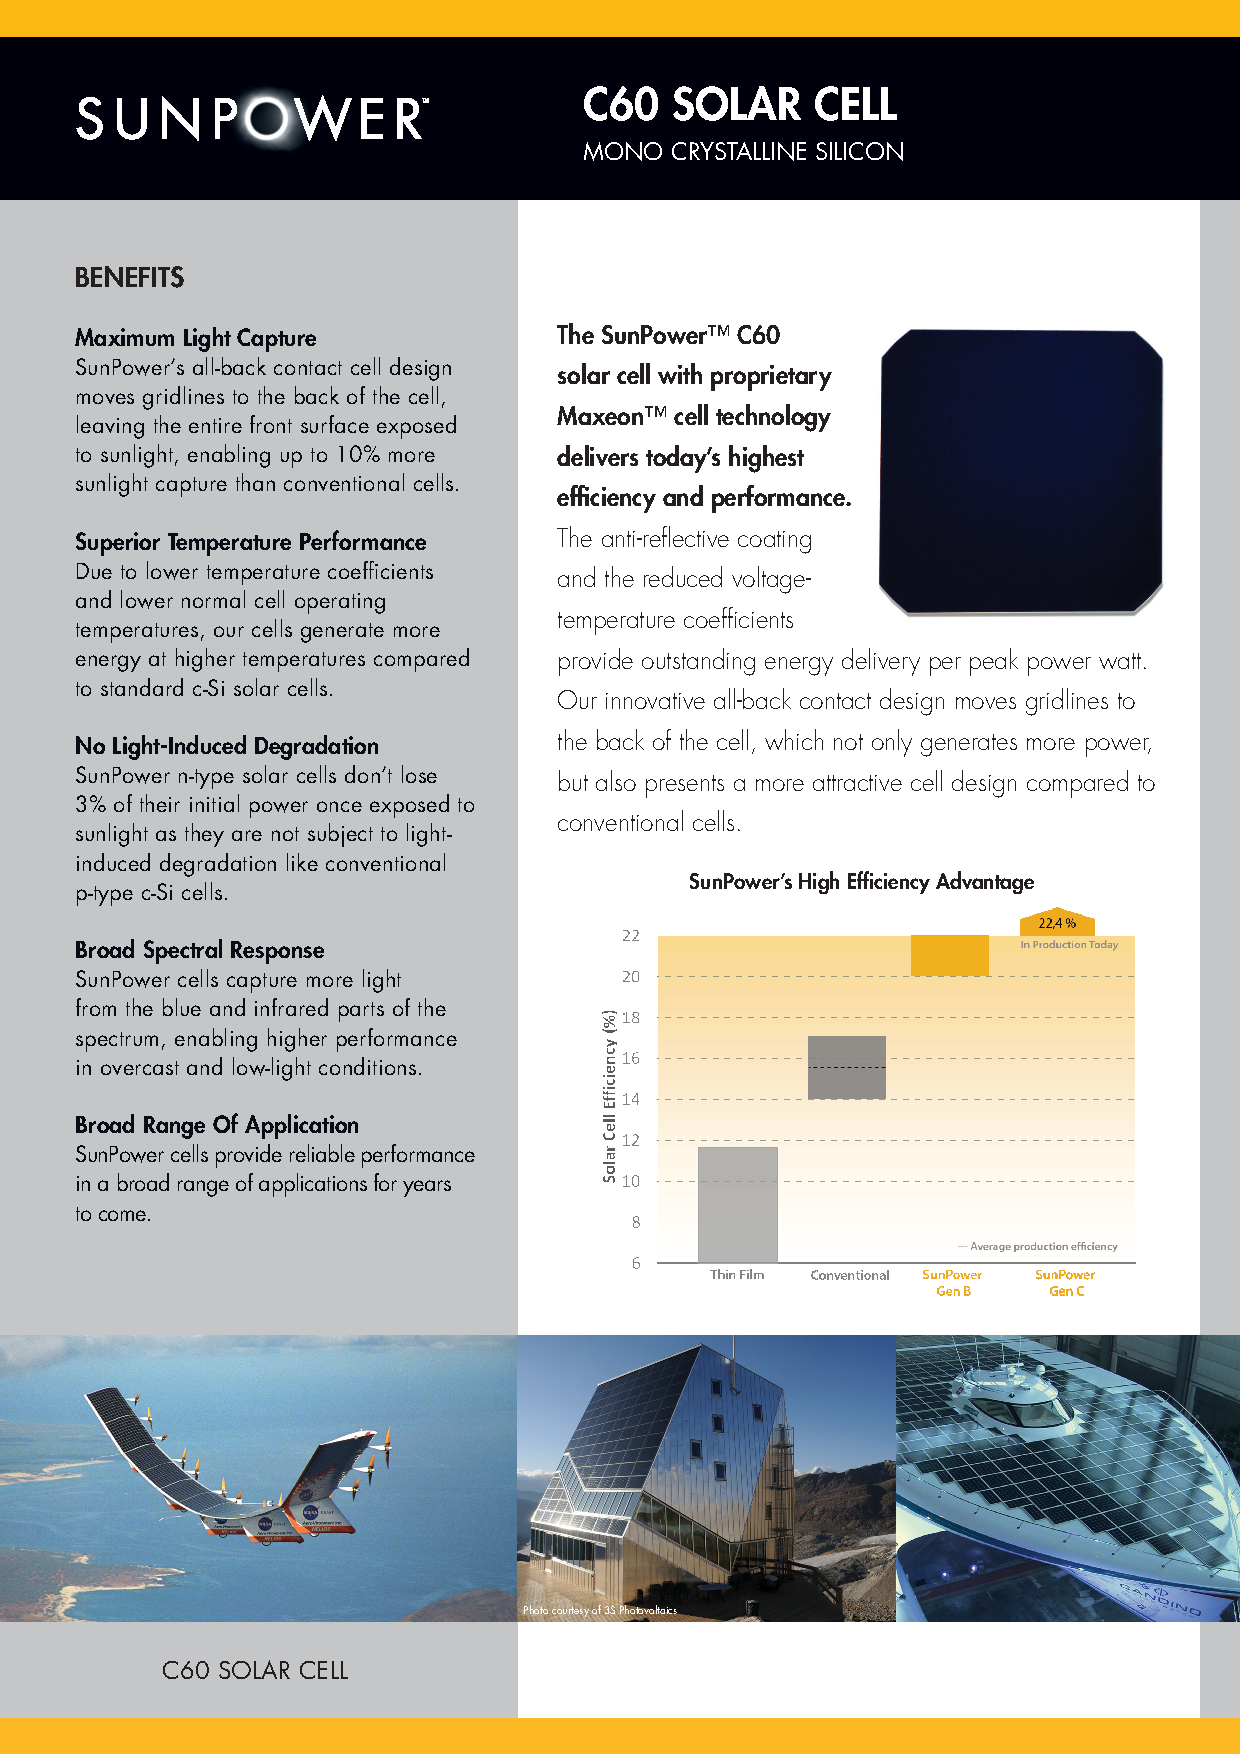
\includepdf[pages={1-2},nup=1x2,landscape=true]{Figures/SolarCell_Sunpower_C60.pdf}

 % file "Thesis_Appendix_B.tex"
%\cleardoublepage

% ----------------------------------------------------------------------
\end{document}
% ----------------------------------------------------------------------

